\documentclass[11pt,a4paper]{report}
\setlength{\textwidth}{165mm}
\setlength{\textheight}{232mm}

\setlength{\oddsidemargin}{0mm}
\setlength{\evensidemargin}{0mm}
\setlength{\topmargin}{-5mm}
\usepackage{cite}
\usepackage{url}
\usepackage{atbegshi}
%\AtBeginShipoutFirst{\special{pdf:tounicode 90ms-RKSJ-UCS2}} % for Shift JIS
\usepackage{amsmath,amssymb}
\usepackage{graphicx}
%\usepackage[dvipdfmx]{graphicx}
\usepackage{tabularx} 
\usepackage{multicol}
\usepackage{ascmac}
\usepackage{comment}
\usepackage{here}
%\usepackage[dvipdfmx]{color}
%\usepackage[dvipdfmx,bookmarks=true,bookmarksnumbered=true,bookmarkstype=toc]{hyperref}
\usepackage[dvipdfmx,hidelinks]{hyperref}
\usepackage{listings} %,jlisting}
%\lstloadlanguages{[90]Fortran,perl,c}
\renewcommand{\lstlistingname}{List }
\lstset{basicstyle=\small\ttfamily,columns=[l]{fullflexible},%
	keywordstyle={\bfseries \color[cmyk]{1,0,0,0}},%
	breaklines=true,%
        xrightmargin=0pt,%
        xleftmargin=3pt,%
	frame=single,%
	framexleftmargin=2pt,
	framexrightmargin=2pt,
	framesep=5pt,
	numbers=left
}

%%% Fancyheadings
\RequirePackage{fancyhdr}
\pagestyle{fancy}

\fancyhf{}
\addtolength{\footskip}{\baselineskip}
%\fancyhead[LE]{\small\leftmark}  % chapter
%\fancyhead[RO]{\small\rightmark} % section
%\fancyhead[L]{\small\leftmark}  % chapter
\fancyhead[R]{\small\rightmark} % section
\fancyfoot[C]{\thepage}
\renewcommand{\headrulewidth}{.4pt}
\renewcommand{\footrulewidth}{.4pt}

\newcommand{\figref}[1]{Figure \ref{#1}}
\newcommand{\tabref}[1]{Table \ref{#1}}
\newcommand{\eref}[1]{Equation(\ref{#1})}
\newcommand{\lstref}[1]{List \ref{#1}}


\title{JcupLT Coupling Library Manual\\
Version 0.5}
\author{JcupLT Developer Team}
\begin{document}
\maketitle

\vspace*{\fill}
\begin{flushright}
\begin{minipage}{0.75\textwidth}
\raggedleft
\large\itshape
``Lo, I am a herald of the lightning,\\
and a heavy drop out of the cloud:\\
the lightning, however, is the \textsc{Superman}.''\\[1em]
\normalsize\upshape
--- Friedrich Nietzsche,\\
\textit{Thus Spoke Zarathustra}
\end{minipage}
\end{flushright}
\vspace*{\fill}
 
\clearpage

\tableofcontents

%================================================================================================
%================================================================================================
%================================================================================================
\chapter*{Preface}

This document is the manual for the coupler JcupLT.
The development of Jcup\cite{Arakawa2011,  Arakawa2020}, the predecessor of JcupLT,
began in 2007 and continues to be improved as of 2026.

During this period, Jcup has been widely adopted as a foundational coupling library primarily for weather and climate models, including the coupling of the atmospheric model NICAM\cite{Satoh2014, Satoh2019} with the ocean model COCO\cite{Miyakawa2017}, the coupling with AI\cite{Arakawa2022}, and the coupling within ILS (Integrated Land Simulator)\cite{Nitta2020}.

However, as its range of applications has expanded,
performance issues have become apparent ---
specifically, the large overhead
associated with data exchange.
This overhead is primarily caused by three factors:
(1) the complexity of internal processing
related to data exchange within Jcup,
(2) the MPI function usage and implementation
for data transmission and reception,
and (3) the interpolation calculation.

To overcome these weaknesses,
a new coupler, JcupLT, has been developed.
The ``LT'' in JcupLT is a double meaning
of \emph{Lightning} and \emph{Lightweight},
implying high speed and low overhead.
JcupLT has three major features:
(1) support for a sufficient set of coupling patterns,
(2) adoption of asynchronous communication,
and (3) realization of send-side interpolation.
These features make it possible to perform
coupling calculations with stringent performance requirements,
such as coupling a high-resolution atmospheric model with ILS.

It is our hope that this manual will help JcupLT
to be widely used
in a diverse range of coupled calculations.

\begingroup
\renewcommand{\chapter}[2]{}  % suppress chapter heading
\bibliographystyle{unsrturl}
%\bibliographystyle{ACM-Reference-Format}
\bibliography{JcupLT}
\endgroup

%================================================================================================
%================================================================================================
%================================================================================================

\chapter{Introduction to Coupled Calculations}

% [Modified] Merged two sentences into one; removed redundant phrasing.
This chapter provides an overview of coupled calculations.
Readers already familiar with coupled calculations may skip this chapter.

% [Modified] "physical aspects" -> consistent use; reworded for conciseness.
First, the physical aspects of coupled calculations are described.
Weather and climate result from the interaction of multiple physical components,
such as the atmosphere and ocean.
% [Modified] Active voice; added latent heat as example; clarified direction.
For example, the atmosphere transfers momentum to the ocean surface,
while the ocean surface transfers sensible and latent heat
to the lower atmosphere (\figref{fig:ao_interaction}).
% [Modified] "Therefore, in a simulation model expressing these phenomena"
%  -> simplified.
A simulation model that represents these phenomena
must therefore exchange the corresponding physical quantities between components.
% [Modified] "At this time" -> "In such a simulation"; simplified verb phrase.
In such a simulation, each component model uses its own grid system and time step
suited to the physical phenomena it represents.
% [Modified] Simplified; replaced "having mutually different" with "with different".
To exchange data between models with different grid systems and time steps,
appropriate time management and grid remapping are required.

\begin{figure}[H]
\begin{center}
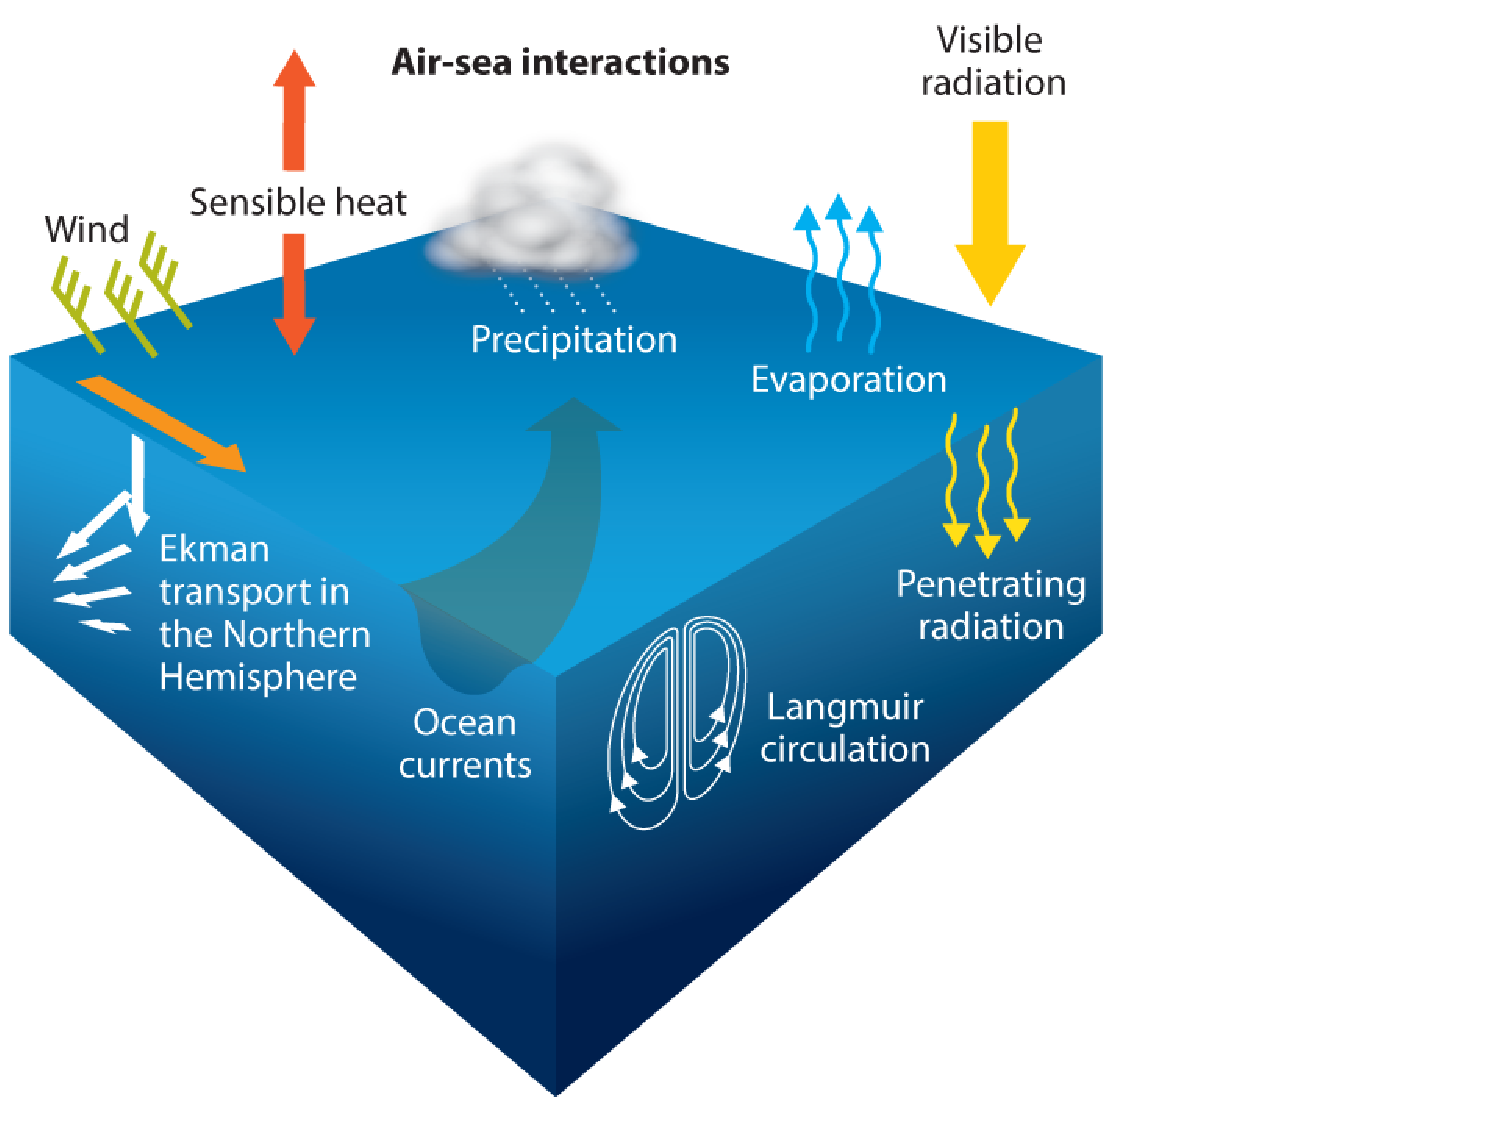
\includegraphics[bb = 0 0 600 550, scale=0.45, clip]{figs/ao_interaction.pdf}
% [Modified] "Schematics" -> "Schematic"; sentence case; \url{} for URL.
\caption{Schematic of atmosphere--ocean interaction
(from Encyclopedia of the Environment, https://www.encyclopedie-environnement.org/en/air-en/biosphere-hydrosphere-and-cryosphere-models/).}
\label{fig:ao_interaction}
\end{center}
\end{figure}

% [Modified] "a computational aspect" -> "the computational aspects" for consistency.
Next, the computational aspects of coupled calculations are described.
% [Modified] "a plurality of arithmetic units" -> "multiple processing units".
Modern high-performance computers operate multiple processing units in parallel.
% [Modified] "correspond to" -> "be designed to exploit".
When running a simulation model on such a computer,
the model must be designed to exploit the computer's parallel architecture.
% [Modified] Simplified sentence structure.
This is generally achieved through domain decomposition,
in which the model grid is divided among processing units.
% [Modified] "a plurality of models" -> "multiple models";
%  "conduct a data exchange" -> "exchange data".
In a coupled calculation, multiple models run in parallel.
Therefore, data exchange must be performed
between the appropriate processes of each model,
taking into account their respective domain decompositions.

\figref{fig:data_exchange_example} shows an example of such a data exchange.
% [Modified] Tightened sentence; removed unnecessary "Here, it is assumed that".
In this example, model~A has an $8 \times 8$ grid divided into $4 \times 4$ regions,
and model~B has a $12 \times 12$ grid divided into $3 \times 3$ regions.
Each region is numbered as shown in the figure.
As indicated by the light green arrow,
region~5 of model~A exchanges data with regions~0, 1, 3, and~4 of model~B.
Conversely, as indicated by the dark green arrows,
region~4 of model~B exchanges data with regions~6, 7, 10, and~11 of model~A.

% [Modified] "It is inappropriate to make individual software" -> rewritten;
%  merged with the next sentence.
Implementing such complex data exchange individually for each model is impractical.
Instead, dedicated software called a \emph{coupler}
(or \emph{coupling library}) is generally used.
As described above, a coupler performs three main tasks:

\begin{enumerate}
\item Control of data exchange timing
\item Grid remapping
\item Data exchange between appropriate processes
\end{enumerate}

\begin{figure}[H]
\begin{center}
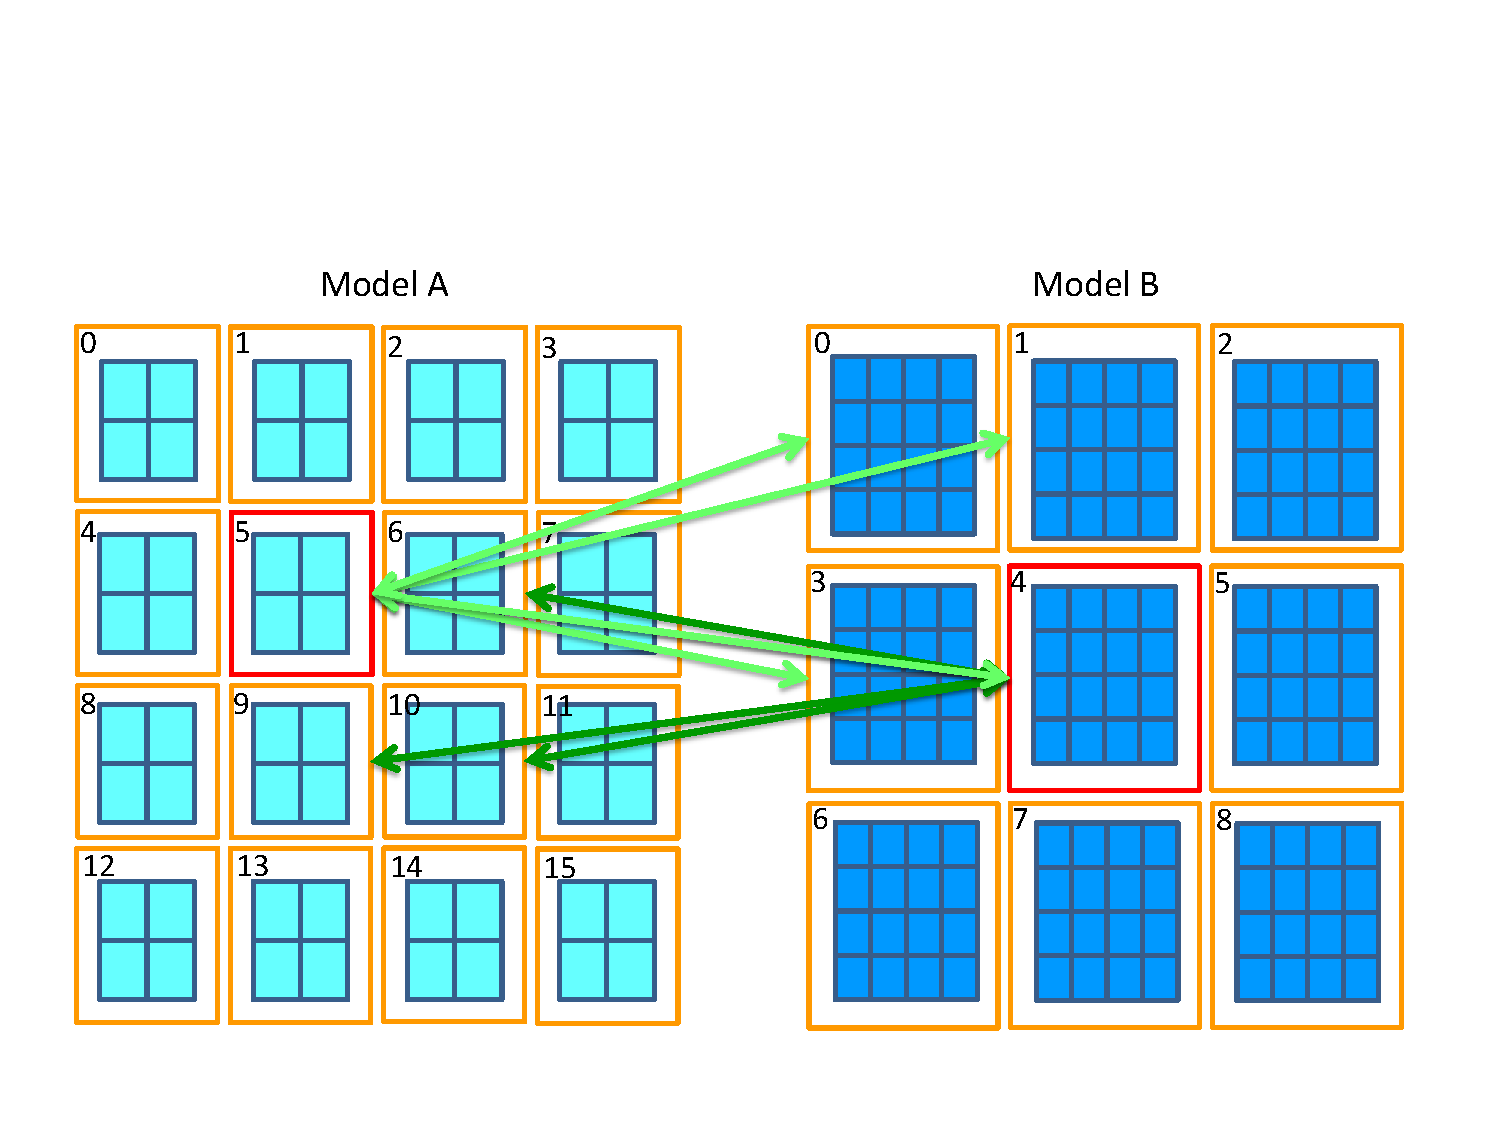
\includegraphics[bb = 0 30 700 450, scale=0.6, clip]{figs/data_exchange_example.pdf}
% [Modified] Added period for consistency.
\caption{Schematic of data exchange between domain-decomposed models.}
\label{fig:data_exchange_example}
\end{center}
\end{figure}
%================================================================================================
%================================================================================================
%================================================================================================
\chapter{Introduction}

\section{Overview of JcupLT}

JcupLT is a lightweight coupling library
derived from the coupling library Jcup.
While Jcup is a general-purpose coupler
that supports a wide range of coupling configurations,
JcupLT is designed to be simpler and faster,
focusing on the core functionality
needed for typical coupled simulations.

JcupLT requires all coupling parameters
to be specified through API subroutines.
To use JcupLT in a model component,
add \texttt{use jlt\_interface} to the source code.

The main features of JcupLT are as follows:

\begin{itemize}
\item Two or more components can be coupled
\item Components can be coupled in series or in parallel
\item Each component can be parallelized through domain decomposition
\item Any grid system can be used, provided that
      each grid point has a unique index
\item A single component can have multiple grid systems
\item The data exchange interval can be set individually for each variable
\item The number of exchangeable variables is unlimited
\item All coupling parameters are configured through API subroutines,
      without requiring a configuration file
\end{itemize}

\section{Coupling Overview}

\subsection{Model requirements for coupling}

Each component model to be coupled must be either single-process (non-parallel)
or parallelized by domain decomposition.
The domain decomposition pattern must remain fixed throughout the simulation,
and the grid point indices assigned to each subdomain must not change.
Grid point indices must be unique across the entire model grid
but do not need to be consecutive.

The data exchange interval for each variable is fixed
and must be an integer multiple of the model time step.
The model time step outside of data exchange times may vary.

\subsection{Coupling pattern}

JcupLT supports coupling two or more component models
in series or in parallel.
Here, \emph{serial coupling} refers to a pattern
in which two components exchange data within the same time step,
and \emph{parallel coupling} refers to a pattern
in which each component sends data from the current time step
and receives data from the previous time step of the other component.

\figref{fig:coupling_pattern} illustrates both patterns.

In the serial coupling example (left),
model~A passes its results to model~B within the same time step,
and model~B then performs its calculation using those results.
Because each component waits for the other to finish,
the total execution time is approximately the sum
of the individual execution times.

In the parallel coupling example (right),
each component sends its results to the other component at each time step
and receives results from the other component at the next time step.
In this case, the total execution time is approximately
that of the slowest component.

The gray squares before $T_0$ represent the initial value exchange.

\begin{figure}[H]
\begin{center}
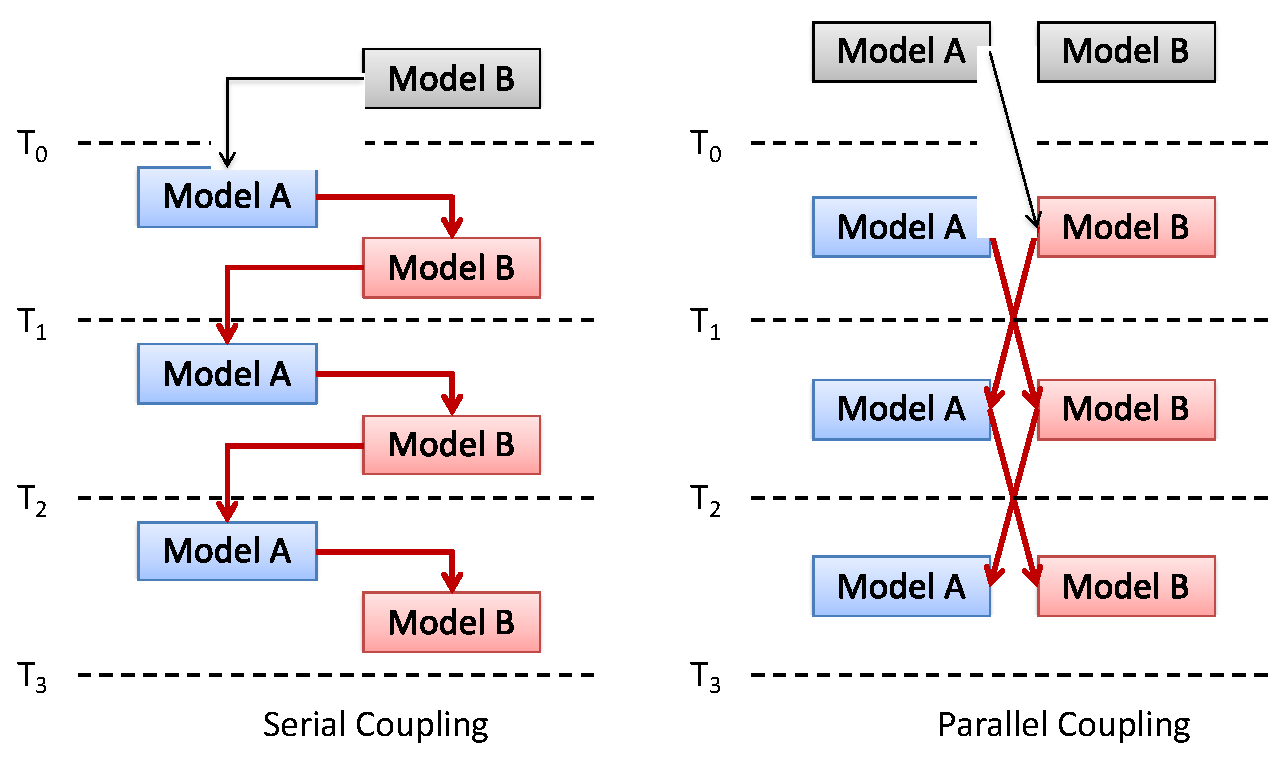
\includegraphics[width=0.8\textwidth]{figs/coupling_pattern.eps}
\caption{Coupling patterns (left: serial coupling, right: parallel coupling).}
\label{fig:coupling_pattern}
\end{center}
\end{figure}

%================================================================================================
%================================================================================================
%================================================================================================
\chapter{Preparation}

\section{Grid index table}

During a coupled calculation,
the coupler must determine which MPI process of the target component
should exchange data with each grid point.
This is determined by two pieces of information:
the grid point index assigned to each subdomain of the component model,
and the remapping table described in the next section.

The grid point indices assigned to each subdomain
are registered with the coupler
through the API subroutine \texttt{jlt\_def\_grid}.

Indices must be positive integers.
They do not need to be contiguous; non-contiguous values are allowed.
However, indices must be unique across all subdomains of the component.
The coupler does not check for duplicates;
if duplicate indices exist, the behavior is undefined.

A single component can have multiple grids,
each with an independent number of grid points and index set.

\section{Remapping table}

JcupLT does not depend on any specific grid structure
and can flexibly couple models whose grids do not change over time.
To achieve this, the correspondence between grid indices of different models
and the associated interpolation coefficients must be prepared in advance.

For example, as shown in \figref{fig:interpolation_image},
the value at grid point $R(p)$ of the receiving model
is calculated from the grid points $S(i)$ to $S(i+4)$
and the corresponding coefficients $C_s(i)$ to $C_s(i+4)$,
as shown in the equation below:

\begin{equation}
R(p) = \sum_{n=0}^{4} C_s(i+n) \cdot S(i+n)
\end{equation}

The remapping table entry for $R(p)$
can be expressed as \lstref{list:mapping_table_sample}.
These values can be calculated
by a remapping table generation tool such as SPRING.
For more information about SPRING,
see https://hydro.iis.u-tokyo.ac.jp/~akira/page/Products/contents/SPRING/v01.03.02/.

In JcupLT, the remapping table is registered with the coupler
through the API subroutine \texttt{jlt\_set\_mapping\_table}.
The sending grid indices, receiving grid indices,
and interpolation coefficients are passed as arrays
to this subroutine.
Details of the API usage are described in a later chapter.

\begin{figure}[H]
\begin{center}
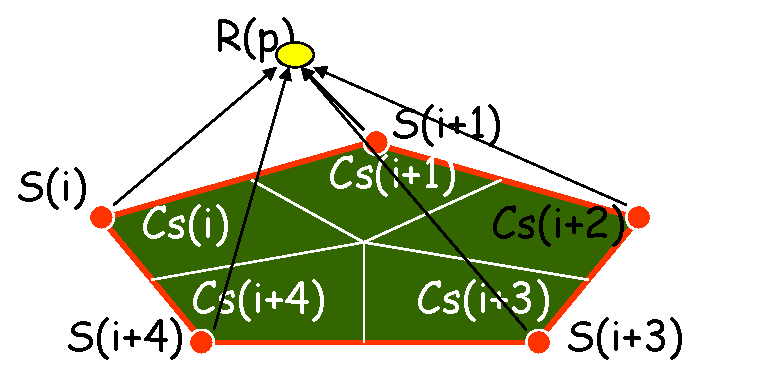
\includegraphics[width=0.8\textwidth]{figs/interpolation_image.eps}
\caption{Grid point indices and interpolation coefficients.}
\label{fig:interpolation_image}
\end{center}
\end{figure}

\begin{lstlisting}[caption=Example of a remapping table entry,
                    label=list:mapping_table_sample]
 R(p), S(i),   Cs(i)
 R(p), S(i+1), Cs(i+1)
 R(p), S(i+2), Cs(i+2)
 R(p), S(i+3), Cs(i+3)
 R(p), S(i+4), Cs(i+4)
\end{lstlisting}


%================================================================================================
%================================================================================================
%================================================================================================

\chapter{How to Use the API Subroutines}

\section{Overview of API usage}

To use JcupLT in a model component,
link the JcupLT library and module files
and add \texttt{use jlt\_interface} to the source code.
The JcupLT API subroutines are divided into four categories:
initialization,
processing before time integration,
processing during time integration,
and finalization.

\section{Initialization}

\subsection{Overview of initialization}

A typical sequence of JcupLT API calls during initialization
is shown in \figref{fig:initialization_process}.
First, initialize JcupLT with \texttt{jlt\_initialize}.
Next, obtain the MPI parameters
generated by JcupLT
using \texttt{jlt\_get\_mpi\_parameter}.
Then, register the grid point indices for each subdomain
with \texttt{jlt\_def\_grid},
and notify JcupLT of the end of grid definition
with \texttt{jlt\_end\_grid\_def}.
After that, register the remapping tables
with \texttt{jlt\_set\_mapping\_table}
and configure the exchange data
with \texttt{jlt\_set\_data}.

\begin{figure}[H]
\begin{center}
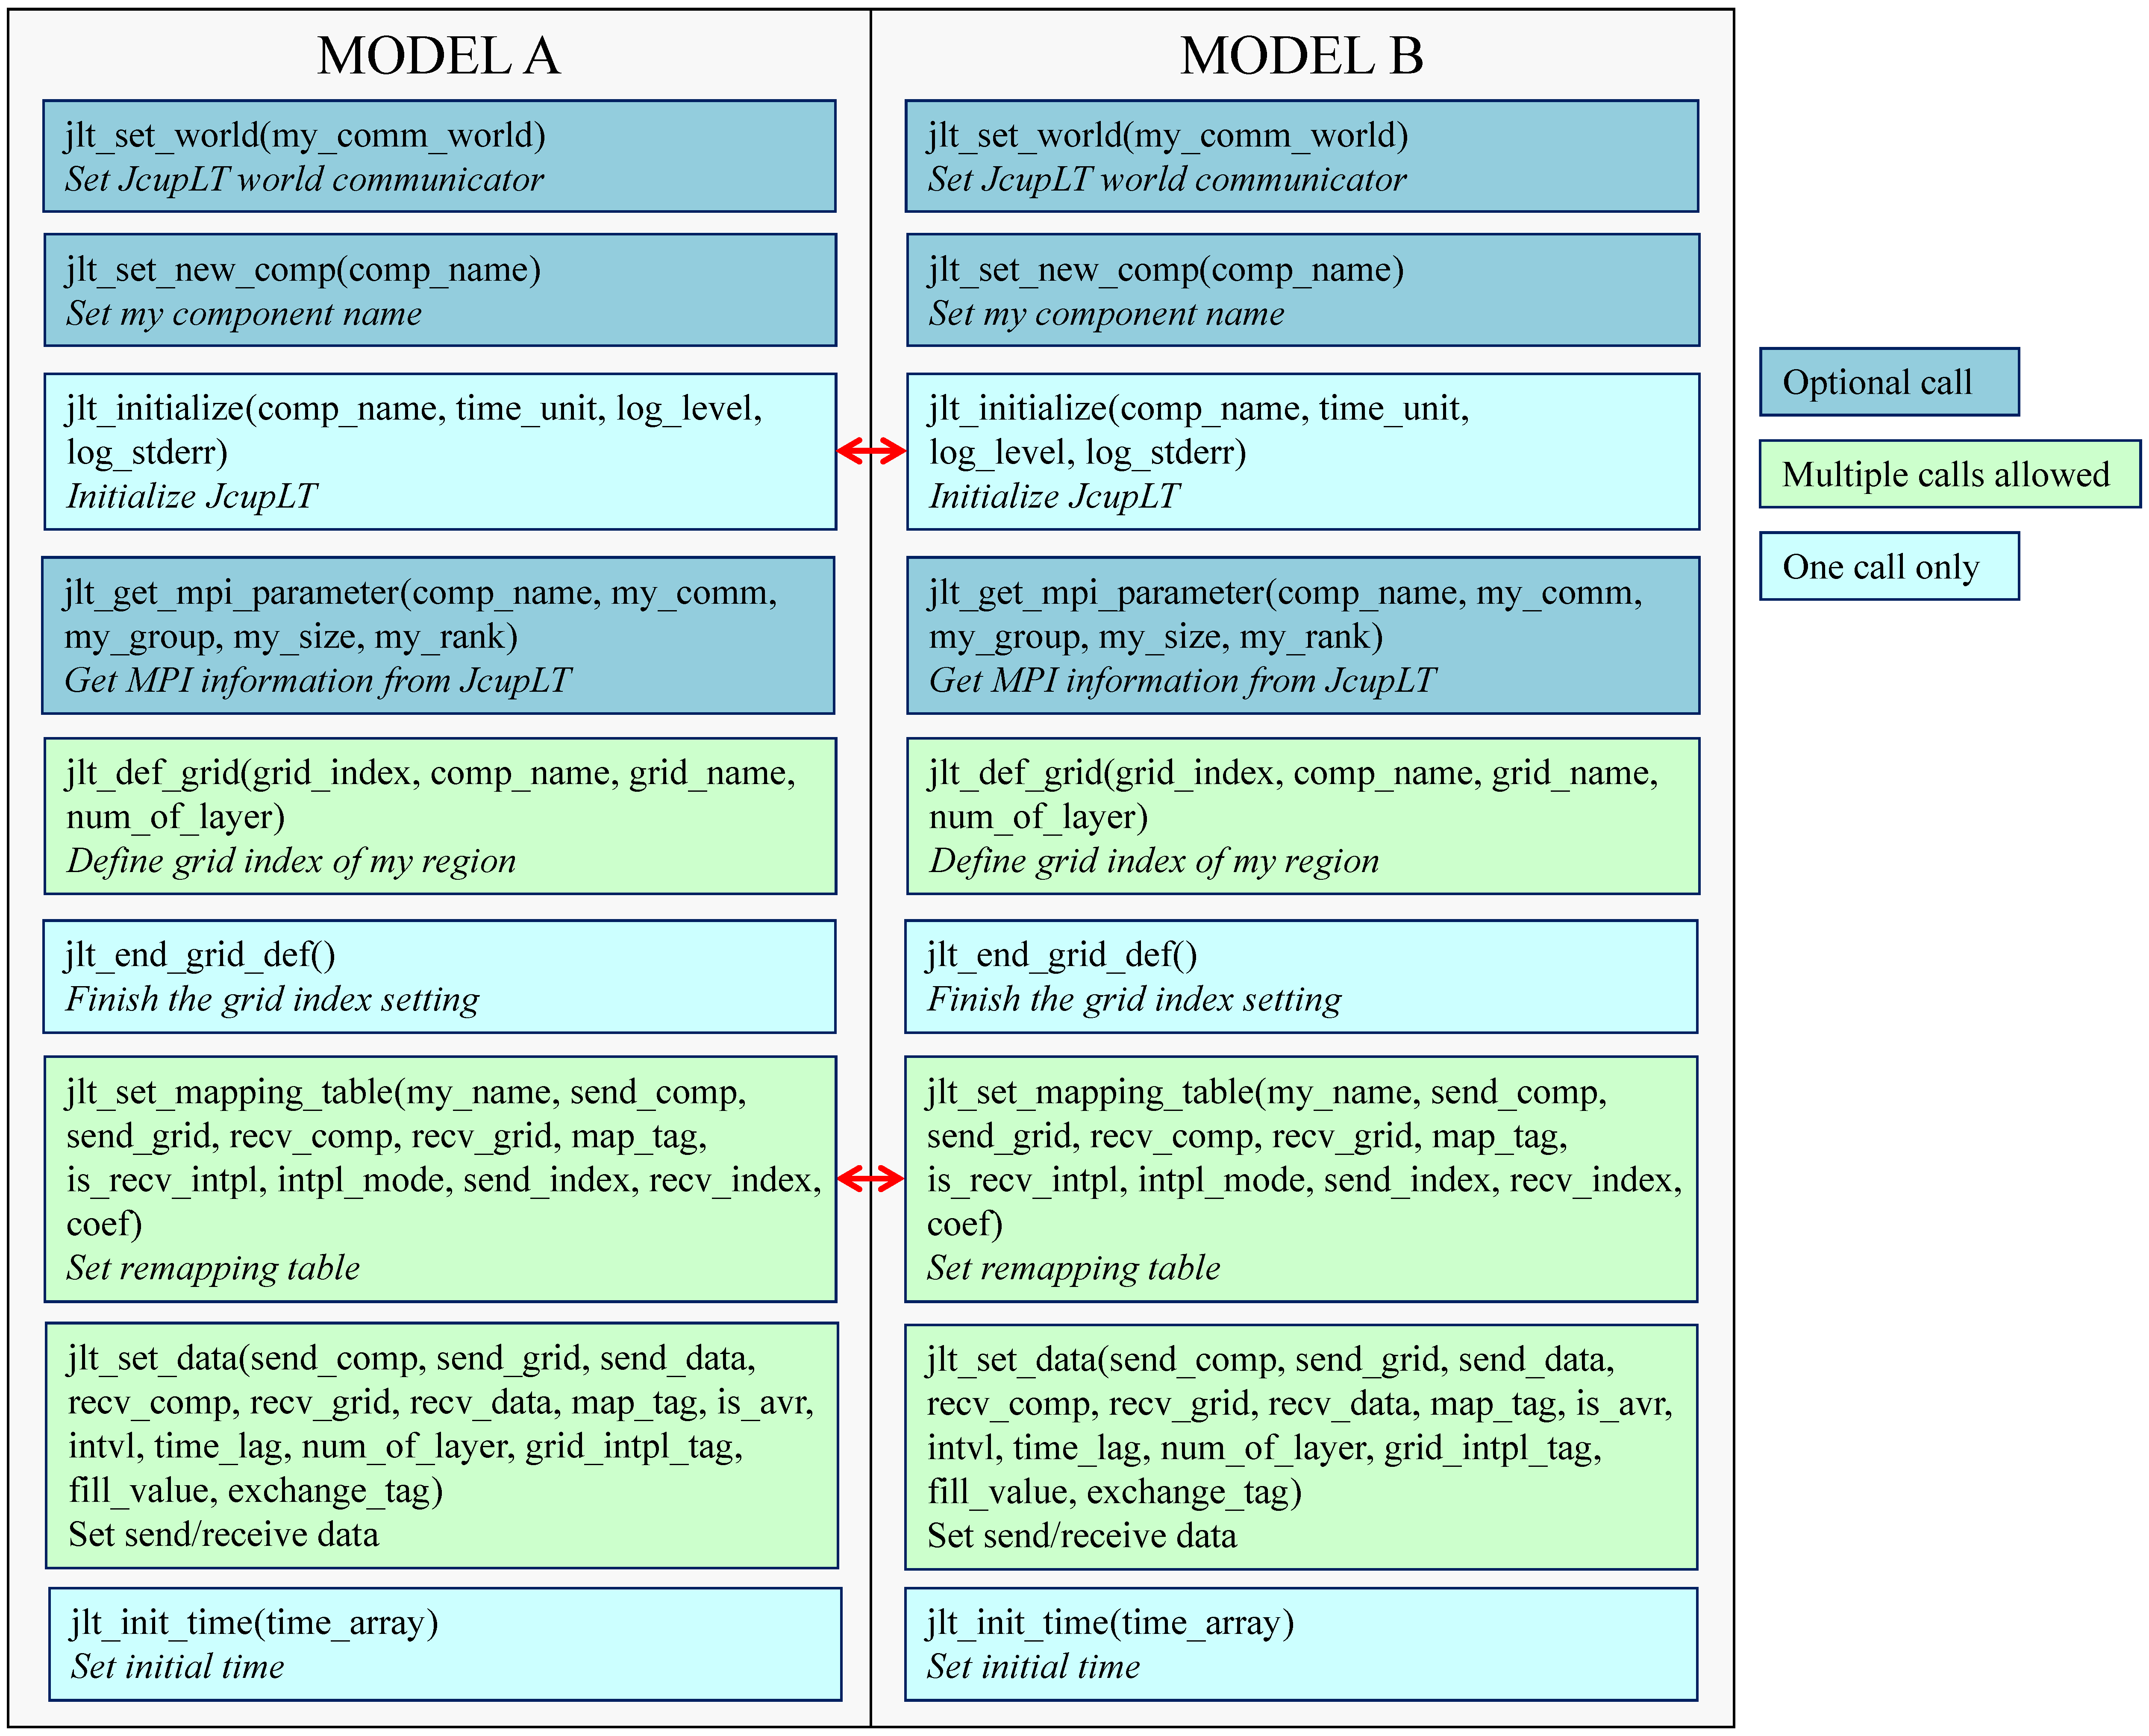
\includegraphics[width=0.8\textwidth]{figs/initialization_process.eps}
\caption{Typical sequence of JcupLT API calls during initialization.}
\label{fig:initialization_process}
\end{center}
\end{figure}

\subsection{Pre-initialization}

As shown in \figref{fig:initialization_process},
two subroutines, \texttt{jlt\_set\_world}
and \texttt{jlt\_set\_new\_comp},
can be called before the initialization routine \texttt{jlt\_initialize}.

\texttt{jlt\_set\_world} is required only when
three or more components are coupled
and only a subset of them use JcupLT for coupling.
In such a case, a dedicated MPI communicator
must be created for the JcupLT-coupled components.
The user must generate this communicator in advance
using the MPI function \texttt{MPI\_Comm\_split},
and pass it to JcupLT via \texttt{jlt\_set\_world}.

\texttt{jlt\_set\_new\_comp} is used
when a single executable contains two or more components.
It registers the second and subsequent component names with JcupLT.
The first (i.e., primary) component name
is set automatically in the initialization subroutine
\texttt{jlt\_initialize}.

Both of these subroutine calls can be omitted
when they are not needed.

\subsection{Initialize JcupLT}

Call \texttt{jlt\_initialize} to initialize JcupLT.
The arguments are as follows:
a character string representing the component name,
a character string representing the time unit,
an integer specifying the log output level,
and a logical flag indicating whether log messages
are also written to standard error output.

The time unit can be one of three values:
\texttt{"SEC"} (seconds),
\texttt{"MIL"} (milliseconds),
or \texttt{"MCR"} (microseconds).
This unit applies to the $\Delta T$ argument
of the time-setting subroutine \texttt{jlt\_set\_time},
described later.

The log output level takes one of three integer values:
0 (no log output),
1 (brief log output),
or 2 (detailed log output).
When the log level is set to 1 or 2,
log messages are written to a file named
\texttt{jlt.\textit{model\_name}.coupling.log.PE??????}.

The last argument accepts \texttt{.true.} or \texttt{.false.}.
When set to \texttt{.true.}
and the log level is 1 or 2,
the same log messages are also written
to standard error output.

\subsection{Get MPI information}

As shown in \figref{fig:mpi_communicator},
when components are coupled through JcupLT,
the MPI communicator for each component
is generated internally by JcupLT.
Therefore, each component must use
the JcupLT-generated communicator
when calling MPI routines.

The MPI parameters for each component
can be obtained by calling \texttt{jlt\_get\_mpi\_parameter}.
The arguments are:
the component name (input),
the local communicator (output),
the local MPI group ID (output),
the number of local MPI processes (output),
and the local MPI rank number (output).

This subroutine call is optional,
but must be called if the component
requires parallel computing information.

\begin{figure}[H]
\begin{center}
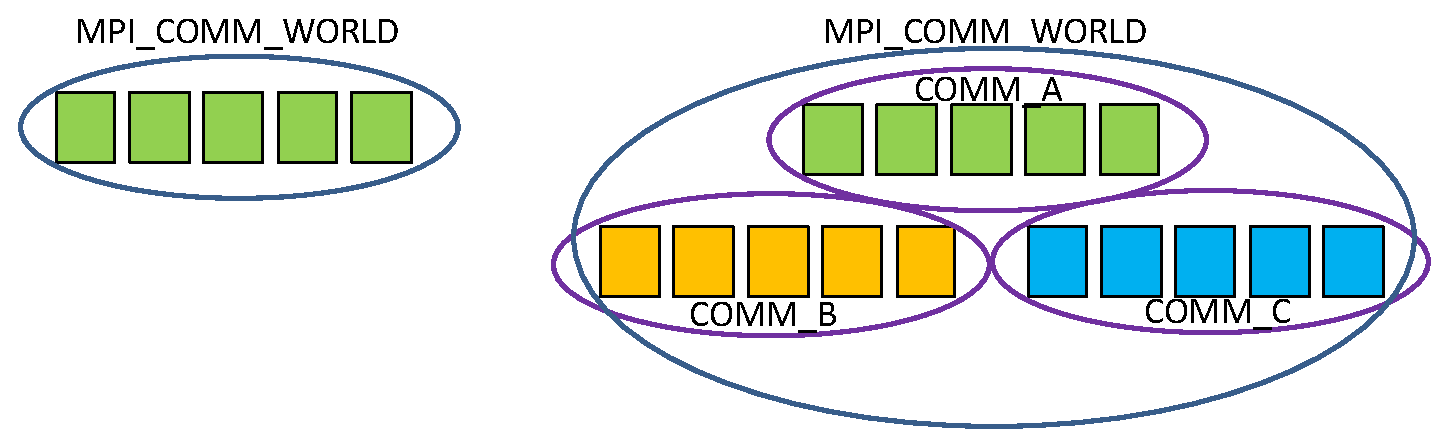
\includegraphics[width=0.8\textwidth]{figs/mpi_communicator.eps}
\caption{MPI communicator layout:
  standalone (left) vs.\ coupled with JcupLT (right).}
\label{fig:mpi_communicator}
\end{center}
\end{figure}

\subsection{Set grid index}

Call \texttt{jlt\_def\_grid} to register the grid point indices
for each subdomain of the component.
The arguments are:
a one-dimensional integer array \texttt{grid\_index(:)}
containing the grid point indices,
a character string \texttt{comp\_name} specifying the component name,
a character string \texttt{grid\_name} specifying the grid name,
and an optional integer \texttt{num\_of\_vgrid}
specifying the number of vertical layers.

The grid point indices are always passed
as a one-dimensional array,
regardless of the actual grid structure.
The grid size is determined
from the size of the \texttt{grid\_index} array.

An important consideration is whether the vertical dimension
should be included in the grid index array.
In many cases, such as atmosphere--ocean coupling,
the exchanged data are horizontally two-dimensional.
Even when a third dimension exists,
it often represents a category rather than
a physical vertical layer.
Furthermore, even when exchanging data
in a physical three-dimensional space
(e.g., atmosphere--chemistry coupling),
the grids may differ only in the horizontal plane,
making vertical interpolation unnecessary.

In these cases, even if the exchanged data have vertical layers,
provide \texttt{grid\_index}
as a horizontally indexed array
and specify the number of vertical layers
via the optional argument \texttt{num\_of\_vgrid}
or via the \texttt{num\_of\_layer} argument
of \texttt{jlt\_set\_data} (described later).
The rules are summarized as follows:

\begin{itemize}
\item When the exchanged data are horizontally 2D,
  or when interpolation is performed
  only in the horizontal plane:
  provide \texttt{grid\_index}
  as a horizontally indexed array
  and specify the number of vertical layers
  through \texttt{num\_of\_vgrid} or \texttt{jlt\_set\_data}.
\item When interpolation is performed in 3D
  including the vertical:
  provide \texttt{grid\_index}
  as an array that includes the vertical dimension.
\end{itemize}

This subroutine can be called multiple times
if the component uses more than one grid system.
After all grids have been registered,
call \texttt{jlt\_end\_grid\_def}
to notify JcupLT that the grid definition is complete.

\subsection{Remapping table setting}

Call \texttt{jlt\_set\_mapping\_table}
to register the remapping table with JcupLT.
The arguments are:
the local component name,
the sending component name,
the sending grid name,
the receiving component name,
the receiving grid name,
a table identification tag,
an interpolation-side flag,
an interpolation-mode string,
the sending grid index array,
the receiving grid index array,
and the coefficient array.

The table identification tag is used
to distinguish multiple remapping tables
defined for the same pair of components and grids.

The interpolation-side flag
takes \texttt{.true.} or \texttt{.false.}.
When set to \texttt{.true.},
the interpolation calculation is performed
on the receiving component;
when set to \texttt{.false.},
it is performed on the sending component.
Note that with send-side interpolation,
results may differ at the level of significant digits
when the number of processes changes.
With receive-side interpolation,
whether binary reproducibility is maintained
depends on the interpolation mode described below.

The interpolation-mode string
takes one of the following values:
\texttt{"FAST"}, \texttt{"SAFE"},
\texttt{"PARALLEL"}, or \texttt{"USER"}.
The first three modes use
the interpolation routines built into JcupLT.
\texttt{"FAST"} processes the remapping table
as simply as possible;
however, results may change
when the number of processes changes.
\texttt{"SAFE"} guarantees that results
do not change with the number of processes.
\texttt{"PARALLEL"} uses OpenMP parallelization
for the interpolation calculation.
\texttt{"USER"} specifies that
a user-defined interpolation subroutine is used.
The user-defined subroutine is registered
through a JcupLT API routine,
described in a later section.

Note that this subroutine involves communication
between the sending and receiving sides.
Therefore, when registering multiple remapping tables,
the order of registration must be consistent
between the sending and receiving components.

\subsection{Exchange data setting}

Call \texttt{jlt\_set\_data}
to configure the information for each exchange variable.
The arguments are:
the sending component name,
the sending grid name,
the sending data name,
the receiving component name,
the receiving grid name,
the receiving data name,
a table identification tag,
a time-averaging flag,
the data exchange interval,
a time lag,
the number of vertical layers,
a data identification tag,
a fill value,
and a data exchange identification tag.

The table identification tag
must correspond to the tag used
in \texttt{jlt\_set\_mapping\_table}.

The time-averaging flag
takes \texttt{.true.} or \texttt{.false.}.
When set to \texttt{.true.},
the data are averaged over the exchange interval.
When set to \texttt{.false.},
the data at the exchange time step
are sent and received directly.

The time lag is set as a pair of values
on the sending and receiving sides.
The following combinations are allowed:

\begin{description}
\item[$(0, 0)$:]
  Immediate data exchange mode.
  In this mode, the \texttt{jlt\_put\_data}
  and \texttt{jlt\_get\_data} calls
  (described later) perform communication synchronously
  on the spot.
  This setting is mainly used
  for exchanging initial values and boundary conditions
  before time integration.
\item[$(-1, -1)$:]
  Parallel execution mode,
  in which two models run concurrently
  and exchange data.
  This is the standard setting for JcupLT.
\item[$(1, -1)$ or $(-1, 1)$:]
  Serial execution mode,
  in which two models run sequentially.
  The component with $-1$ is the preceding model.
\end{description}

The number of vertical layers
specifies the vertical extent of the data.

The data identification tag
is used to identify the variable
during interpolation calculations
and is referenced by user-defined interpolation subroutines.

The fill value specifies the value
to be excluded from the calculation
when computing time-averaged data.

The data exchange identification tag
is passed to the MPI communication functions.
The MPI functions use this tag
to match the appropriate sender and receiver.

\texttt{jlt\_set\_data} must be called
on both the sending and receiving sides,
although the order of calls
may differ between the two sides.

\subsection{Set initial time}

Call \texttt{jlt\_init\_time} to set the initial time.
The argument is an integer array of size~6,
representing year, month, day, hour, minute, and second.

\section{Processing before time integration}

\subsection{Overview of preprocessing}

Before entering the time integration loop,
initial values and other necessary information
can be exchanged between components.
In addition, the initial time must be set,
and data that will be received
at the first time step must be put before entering the loop.
An overview of these API calls
is shown in \figref{fig:pre_integration_process}.

\begin{figure}[H]
\begin{center}
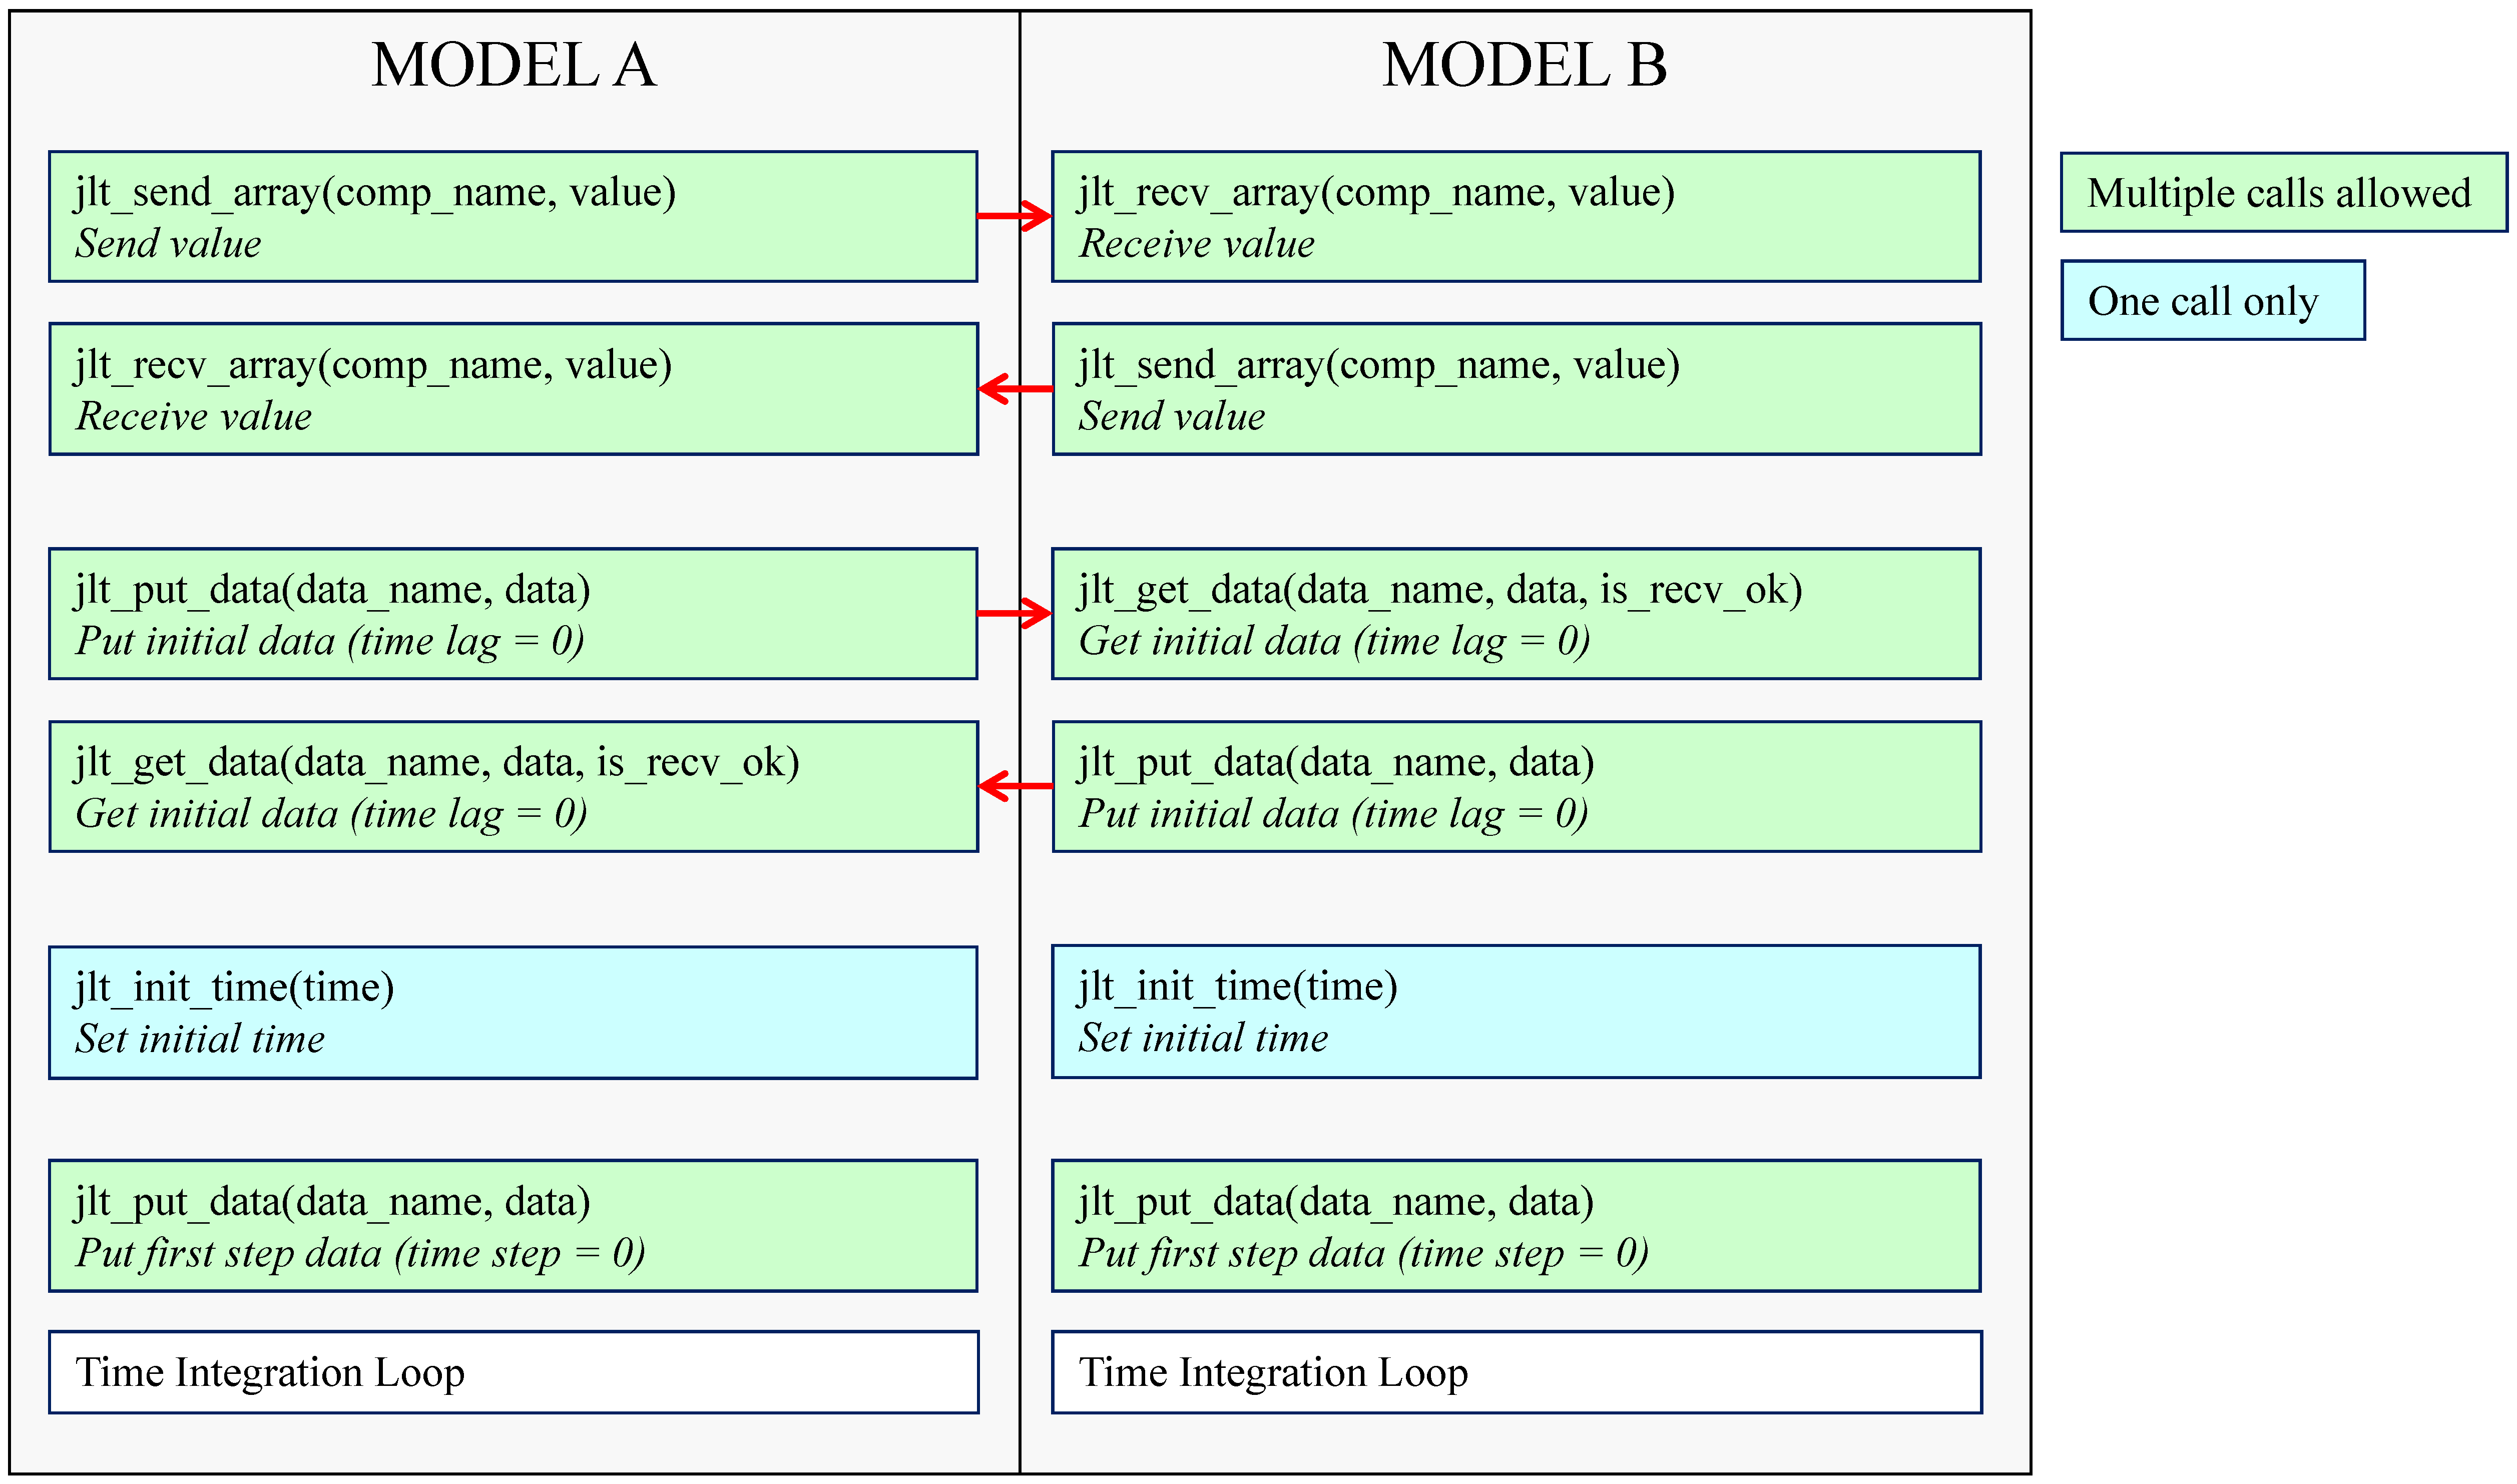
\includegraphics[width=0.8\textwidth]{figs/pre_integration_process.eps}
\caption{Typical sequence of JcupLT API calls
  before the time integration loop.}
\label{fig:pre_integration_process}
\end{center}
\end{figure}

\subsection{Exchange of miscellaneous information}

To exchange miscellaneous information before time integration
(e.g., integration start time),
use \texttt{jlt\_send\_array} and \texttt{jlt\_recv\_array}.
The arguments are the name of the other component
and the value to communicate.
The value argument can be
a string, integer array,
real (single-precision) array,
or double-precision array.
The send and receive calls must correspond to each other.

\subsection{Exchange of initial data}

To exchange initial grid data
(e.g., boundary conditions or static fields)
before the time integration loop,
use \texttt{jlt\_put\_data} and \texttt{jlt\_get\_data}
for variables whose time lag is set to~0
in \texttt{jlt\_set\_data}.
In this mode, communication is performed synchronously:
\texttt{jlt\_put\_data} on the sending side
and \texttt{jlt\_get\_data} on the receiving side
must correspond to each other
for all time-lag-0 variables.

\subsection{Set initial time}

If \texttt{jlt\_init\_time} was not called
during the initialization phase (Section~4.2.8),
it must be called here
before entering the time integration loop.
The argument is an integer array of size~6,
representing year, month, day, hour, minute, and second.

\subsection{Put initial values for the first time step}

Before entering the time integration loop,
the sending component must put the data
that the receiving component will obtain at the first time step.
Call \texttt{jlt\_put\_data} with the data name
and the data array as arguments.



\section{Time integration}

\subsection{Overview of time integration}

The JcupLT API calls used in the time integration loop
are shown in \figref{fig:time_loop_process}.
Three API routines are used:
\texttt{jlt\_set\_time},
\texttt{jlt\_get\_data},
and \texttt{jlt\_put\_data}.
All three routines must be called at every time step.

The data flow in JcupLT differs from
that of a simple send-then-receive scheme.
The key points are as follows:

\begin{enumerate}
\item JcupLT allows the interpolation calculation
  to be performed on either the sending or the receiving side.
  Which side performs the interpolation
  is determined by the interpolation-side flag
  set in \texttt{jlt\_set\_mapping\_table}.
  In the example shown in
  \figref{fig:time_loop_process},
  Model~B performs the interpolation.

\item When \texttt{jlt\_put\_data} is called,
  the data are sent immediately
  via non-blocking communication (\texttt{MPI\_Isend}).
  If the current step is not a sending step,
  the coupler skips the send internally.
  Therefore, the user does not need to check
  the step before calling this routine.

\item Data reception (\texttt{MPI\_Irecv}),
  completion of pending send and receive operations,
  and the interpolation calculation
  are all performed internally
  within \texttt{jlt\_set\_time}.
  If there is a load imbalance between components,
  a wait may occur in this subroutine.
\end{enumerate}

\begin{figure}[H]
\begin{center}
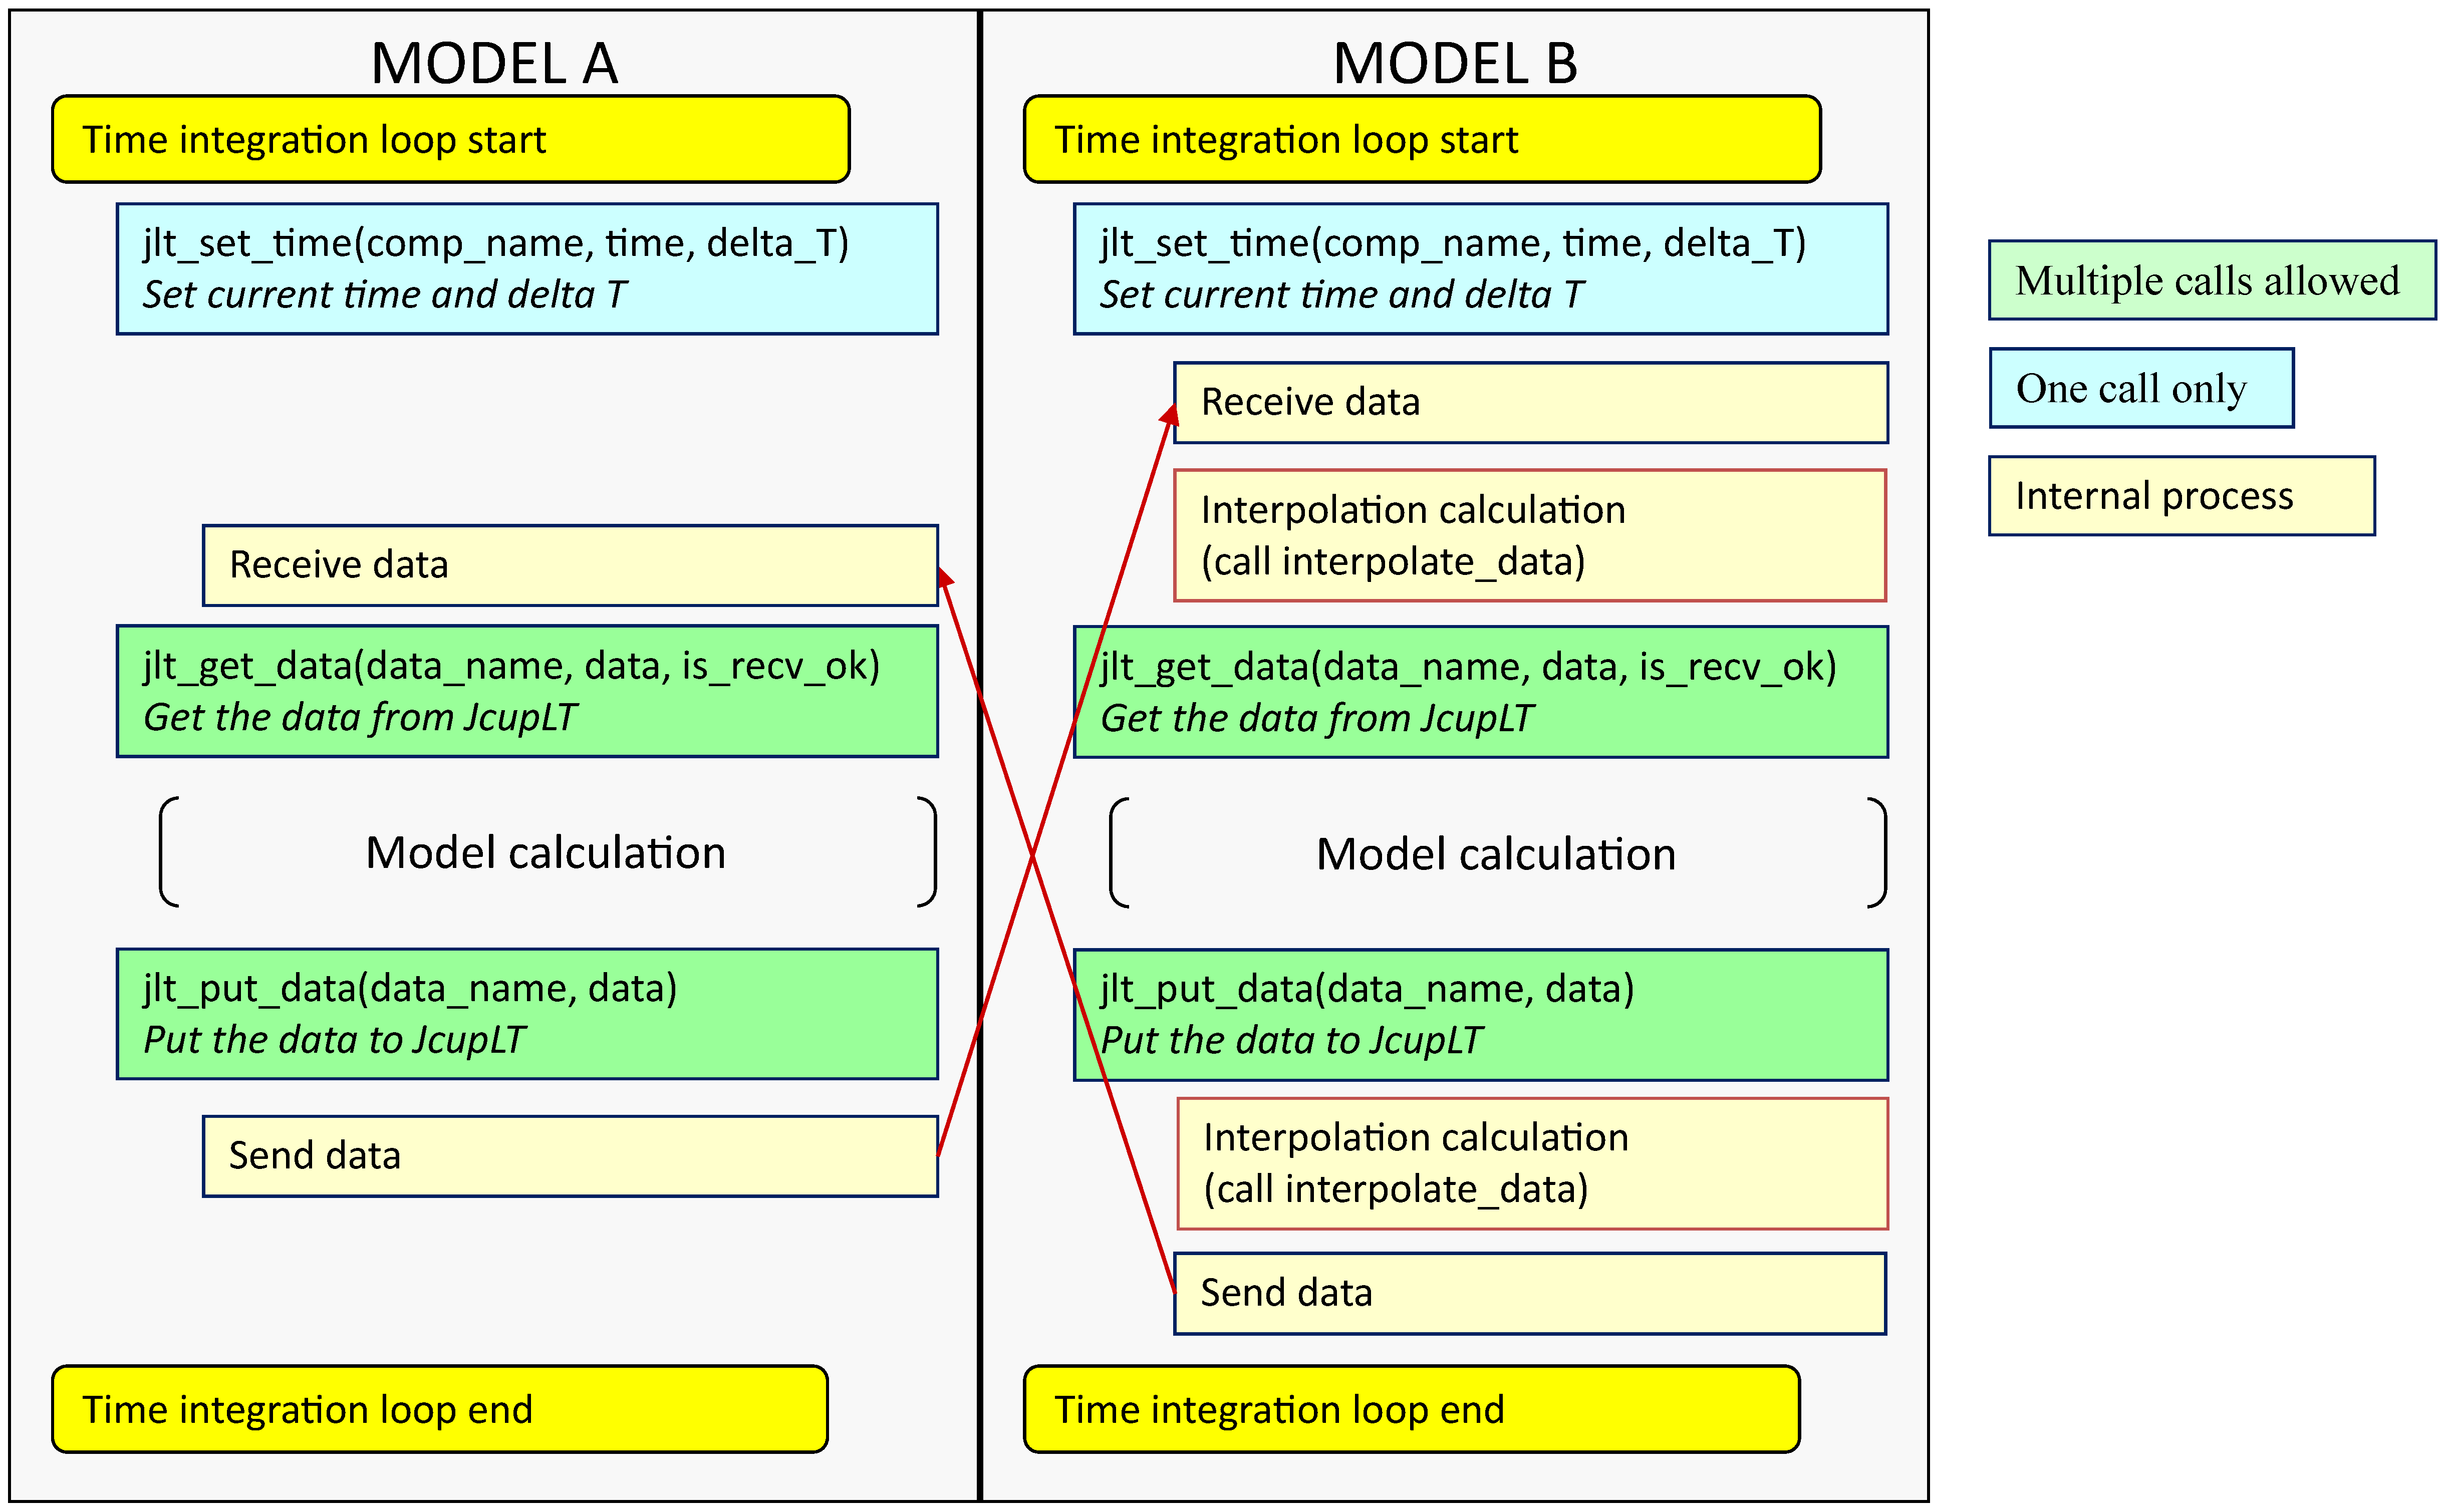
\includegraphics[width=0.8\textwidth]{figs/time_loop_process.eps}
\caption{Typical sequence of JcupLT API calls
  in the time integration loop.
  In this example, Model~B performs
  the interpolation calculation.}
\label{fig:time_loop_process}
\end{center}
\end{figure}

\subsection{Setting the current time and $\Delta T$}

Call \texttt{jlt\_set\_time} at each time step
to pass the component name,
the current time, and $\Delta T$ to JcupLT.
The arguments are a character string
specifying the component name,
an integer array of size~6
(year, month, day, hour, minute, second),
and an integer representing $\Delta T$.
The unit of $\Delta T$ is determined
by the time unit specified
in \texttt{jlt\_initialize}.

Internally, this subroutine performs
data reception, completion of pending communications,
and the interpolation calculation.
Because the coupler uses the accumulated value of $\Delta T$
for data exchange timing,
\texttt{jlt\_set\_time} must be called at every step.

\subsection{Getting data}

Call \texttt{jlt\_get\_data} to obtain exchange data
from JcupLT.
The argument \texttt{data\_name} is the variable name,
and \texttt{data} is the receiving array.
The optional argument \texttt{is\_recv\_ok}
is a logical flag that indicates
whether data were actually received at this call.
Because the data exchange interval
does not necessarily match the model time step,
use this argument to determine
whether new data were received.

\subsection{Putting data}

Call \texttt{jlt\_put\_data} to send data to JcupLT.
The argument \texttt{data\_name} is the variable name,
and \texttt{data} is the sending data array.

When this subroutine is called at a sending step,
the data are dispatched immediately
via non-blocking communication.
If the current step is not a sending step,
the coupler skips the send internally.
Therefore, the user does not need to check
the step before calling this routine.

\section{Finalization}

Call \texttt{jlt\_coupling\_end} at the end of the coupled calculation.
The first argument is an integer array
representing the time at the end of the simulation.
The second argument \texttt{is\_call\_finalize} is a flag
indicating whether \texttt{MPI\_Finalize}
should be called internally by JcupLT.


\section{Other important routines}

\subsection{Error handling routine}

The subroutine \texttt{jlt\_error}
outputs an error message and terminates the program.
The arguments are
a character string \texttt{sub\_name}
specifying the name of the subroutine where the error occurred,
and a character string \texttt{err\_str}
containing the error message.

\subsection{Component query routines}

The function \texttt{jlt\_get\_num\_of\_component}
returns the total number of coupled components.

The function \texttt{jlt\_get\_component\_name}
returns the component name
corresponding to the given component ID number.

The function \texttt{jlt\_get\_comp\_num\_from\_name}
returns the component ID number
corresponding to the given component name.

The function \texttt{jlt\_is\_my\_component}
takes a component name or ID number as input
and returns whether the calling process
belongs to that component.

\subsection{Execution status routine}

The function \texttt{jlt\_is\_model\_running}
returns whether the component
specified by the argument \texttt{comp\_name}
is currently running.

\subsection{MPI information routine}

The function \texttt{jlt\_get\_myrank\_global}
returns the rank number of the calling process
among all coupled processes.

\subsection{Log output routine}

The subroutine \texttt{jlt\_log}
writes a message to the JcupLT log file.
The arguments are
a character string \texttt{sub\_name}
specifying the subroutine name,
a character string \texttt{log\_str}
containing the log message,
and an optional integer \texttt{log\_level}
specifying the log output level.
The log level corresponds to
the log output level set in \texttt{jlt\_initialize}.

\subsection{Calendar routines}

The subroutine \texttt{jlt\_inc\_calendar}
increments a date by a specified number of seconds.
The arguments are
an integer array representing the date
(year, month, day, hour, minute, second)
and an integer \texttt{delta\_t} in seconds.

The subroutine \texttt{jlt\_inc\_time}
increments a date by the $\Delta T$ value
that was given to \texttt{jlt\_set\_time}.
The arguments are the component name
and an integer array representing the date.

\subsection{User-defined interpolation code setting routine}

The subroutine \texttt{jlt\_set\_user\_interpolation}
registers a user-defined interpolation subroutine.
The arguments \texttt{send\_comp} and \texttt{send\_grid}
are the component name and the grid name
on the sending side.
The arguments \texttt{recv\_comp} and \texttt{recv\_grid}
are the component name and the grid name
on the receiving side.
The argument \texttt{map\_tag}
is the remapping table identification tag.
The argument \texttt{user\_func}
is a procedure pointer to the user-defined subroutine.
The details of this subroutine are described
in a later chapter.


%================================================================================================
%================================================================================================
%================================================================================================
\chapter{Implementation of Coupling Code}

\section{Overview of implementation}

This chapter explains how to implement coupling code,
using concrete examples.

\section{Example: toy model}

The first example is a simple toy model,
shown in \lstref{list:code_toy}.
% NOTE: Line numbers below refer to \lstref{list:code_toy}.
%       If the code is modified, verify that these references
%       remain correct.

JcupLT is initialized by calling
\texttt{jlt\_initialize} at line~49,
and MPI information is obtained
via \texttt{jlt\_get\_mpi\_parameter} at line~51.
The grid point indices are calculated in lines~55--69
and registered with \texttt{jlt\_def\_grid} at line~71.
The end of the grid definition
is declared by \texttt{jlt\_end\_grid\_def} at line~73.

The remapping tables are set
by \texttt{jlt\_set\_mapping\_table} at lines~77--80,
and the exchange data are configured
by \texttt{jlt\_set\_data} at lines~82--85.
In this example, two variables are defined:
\texttt{"varc1c2"} sent from COMP1 to COMP2
and \texttt{"varc2c1"} sent from COMP2 to COMP1,
both with a time lag of $-1$ (parallel coupling)
and an exchange interval of 3600 seconds.

The first-step data are put
by \texttt{jlt\_put\_data} at line~93.

Lines~95--107 form the time integration loop.
At the beginning of each iteration,
\texttt{jlt\_set\_time} is called at line~96
to pass the component name,
the current time, and $\Delta T$ to JcupLT.
At line~98, \texttt{jlt\_get\_data} retrieves data,
and at line~104,
\texttt{jlt\_put\_data} sends data.
The calendar is incremented
by \texttt{jlt\_inc\_calendar} at line~106.

The finalization routine \texttt{jlt\_coupling\_end}
is called at line~109.

\begin{lstlisting}[caption=Code of the toy model, label=list:code_toy]
subroutine cal_start_end(num_grid, num_div, my_pos, is, ie)
  implicit none
  integer, intent(IN)  :: num_grid
  integer, intent(IN)  :: num_div
  integer, intent(IN)  :: my_pos
  integer, intent(OUT) :: is, ie
  integer :: div_num

  div_num = num_grid/num_div

  is = div_num * (my_pos - 1) + min(my_pos - 1, mod(num_grid, num_div))
  ie = is + div_num - 1
  if (my_pos <= mod(num_grid, num_div)) ie = ie + 1

  is = is + 1
  ie = ie + 1

end subroutine cal_start_end

program comp1
  use mpi
  use jlt_interface
  implicit none
  integer :: time_array(6) = (/2000,1,1,0,0,0/)
  character(len=64) :: my_name = "COMP1"
  character(len=64) :: my_grid = "COMP1_GRID"
  integer, parameter :: num_grid_global = 12
  integer, parameter :: grid_index_global(num_grid_global) = (/1, 2, 3, 4, 5, 6, 7, 8, 9, 10, 11, 12/)
  !integer, parameter :: grid_index_global(num_grid_global) = (/12, 11, 10, 9, 8, 7, 6, 5, 4, 3, 2, 1/)
  !integer, parameter :: grid_index_global(num_grid_global) = (/1, 3, 5, 7, 9, 11, 2, 4, 6, 8, 10 ,12/)
  integer, parameter :: send_index(num_grid_global) = (/1, 2, 3, 4, 5, 6, 7, 8, 8, 10, 11, 12/)
  integer, parameter :: recv_index(num_grid_global) = (/1, 2, 3, 4, 5, 6, 6, 8, 9, 10, 11, 12/)
  real(kind=8)       :: coef(num_grid_global)
  integer, allocatable :: local_grid_index(:)
  integer :: int_array(1)
  integer :: ierror
  integer :: i
  integer :: my_comm, my_group, my_size, my_rank
  integer :: m, n
  integer :: my_pos_x, my_pos_y
  integer :: is, ie, js, je
  integer :: my_rank_global
  integer :: grid_size
  integer :: num_of_layer = 1
  logical :: is_recv_ok
  real(kind=8), allocatable :: data(:)
  integer :: t

  call jlt_initialize(my_name, "SEC", log_level = 2)

  call jlt_get_mpi_parameter(trim(my_name), my_comm, my_group, my_size, my_rank)

  call mpi_comm_rank(MPI_COMM_WORLD, my_rank_global, ierror)

  m = my_size
  n = 1
  my_pos_x = mod(my_rank, m) + 1
  my_pos_y = my_rank/m + 1

  call cal_start_end(num_grid_global, m, my_pos_x, is, ie)
  call cal_start_end(1, n, my_pos_y, js, je)

  grid_size = ie - is + 1

  allocate(local_grid_index(grid_size))

  do i = 1, grid_size
     local_grid_index(i) = grid_index_global(is+i-1)
  end do

  call jlt_def_grid(local_grid_index, trim(my_name), trim(my_grid), num_of_layer)

  call jlt_end_grid_def()

  coef(:) = 1.0

  call jlt_set_mapping_table(my_name, "COMP1", "COMP1_GRID", &
                                              "COMP2", "COMP2_GRID", 1, .false., "SAFE", send_index, recv_index, coef)
  call jlt_set_mapping_table(my_name, "COMP2", "COMP2_GRID", &
                                             "COMP1", "COMP1_GRID", 1, .false., "SAFE", send_index, recv_index, coef)

  call jlt_set_data("COMP1", "COMP1_GRID", "varc1c2", &
                              "COMP2", "COMP2_GRID", "varc1c2", 1, .false., 3600, -1, 1, 1, -999.d0, 1)
  call jlt_set_data("COMP2", "COMP2_GRID", "varc2c1", &
                              "COMP1", "COMP1_GRID", "varc2c1", 1, .false., 3600, -1, 1, 1, -999.d0, 2)

  allocate(data(grid_size))

  do i = 1, grid_size
     data(i) = is+i-1
  end do

  call jlt_put_data("varc1c2", data)

  do t = 1, 24
     call jlt_set_time(my_name, time_array, 3600)

     call jlt_get_data("varc2c1", data, is_recv_ok = is_recv_ok)

     do i = 1, grid_size
        data(i) = t * 100 + is+i-1
     end do

     call jlt_put_data("varc1c2", data)

     call jlt_inc_calendar(time_array, 3600)
  end do

  call jlt_coupling_end(time_array, .true.)

  stop

end program comp1
\end{lstlisting}



%================================================================================================
%================================================================================================
%================================================================================================
\chapter{Implementation of Interpolation Code}

\section{Overview}
In JcupLT, the basic interpolation routines
are built in by default.
Therefore, unless special requirements exist,
users do not need to implement any interpolation code.

However, if a user needs to apply
a custom interpolation algorithm,
JcupLT provides a mechanism
for calling user-defined subroutines
from within the coupling library.
This chapter describes how to write
and configure such user-defined
interpolation subroutines.

\section{Implementing a user-defined interpolation subroutine}

The interface for a user-defined interpolation subroutine
is defined as shown in \lstref{list:interpolation_user_ifc}.

\begin{description}
\item[\texttt{send\_data}]
  The sending data array.
\item[\texttt{recv\_data}]
  The receiving data array.
\item[\texttt{send\_index}, \texttt{recv\_index}]
  The grid point indices on the sending and receiving sides
  for the interpolation calculation.
\item[\texttt{coef}]
  The interpolation coefficients.
\item[\texttt{num\_of\_layer}]
  The number of vertical layers,
  corresponding to the size of the second dimension
  of \texttt{send\_data} and \texttt{recv\_data}.
\item[\texttt{num\_of\_conv}]
  The size of the interpolation loop,
  corresponding to the array size
  of \texttt{send\_index} and \texttt{recv\_index}.
\item[\texttt{intpl\_tag}]
  The data identification tag value
  defined for each variable
  in \texttt{jlt\_set\_data}.
\end{description}

The user implements the interpolation calculation
using these arguments.
A basic example of an interpolation subroutine
is shown in \lstref{list:example_interpolation_code}.
Note that this calculation is already provided
as the default implementation.
How to register the subroutine with JcupLT
is described in the next section.

\begin{lstlisting}[caption=Interface of user-defined interpolation subroutine,
                    label=list:interpolation_user_ifc]
  abstract interface
    subroutine interpolation_user_ifc(send_data, recv_data, send_index, recv_index, coef, &
                                      num_of_layer, num_of_conv, intpl_tag)
      real(kind=8), intent(IN)     :: send_data(:,:)
      real(kind=8), intent(INOUT)  :: recv_data(:,:)
      integer, intent(IN)          :: send_index(:)
      integer, intent(IN)          :: recv_index(:)
      real(kind=8), intent(IN)     :: coef(:)
      integer, intent(IN)          :: num_of_layer
      integer, intent(IN)          :: num_of_conv
      integer, intent(IN)          :: intpl_tag
    end subroutine
  end interface
\end{lstlisting}

\begin{lstlisting}[caption=Example of a basic interpolation calculation,
                    label=list:example_interpolation_code]
recv_data(:,:) = 0.d0
do l = 1, num_of_layer
  do i = 1, num_of_conv
    sidx = send_index(i)
    ridx = recv_index(i)
    recv_data(ridx, l) = recv_data(ridx, l) + send_data(sidx, l) * coef(i)
  end do
end do
\end{lstlisting}

\section{Registering a user-defined interpolation subroutine}

A user-defined interpolation subroutine
can be registered with the JcupLT API routine
\texttt{jlt\_set\_user\_interpolation}.

The arguments are as follows:

\begin{description}
\item[\texttt{send\_comp}, \texttt{send\_grid}]
  The component name and grid name on the sending side.
\item[\texttt{recv\_comp}, \texttt{recv\_grid}]
  The component name and grid name on the receiving side.
\item[\texttt{map\_tag}]
  The mapping table identification tag.
\end{description}

These values must correspond to the entries
specified in \texttt{jlt\_set\_mapping\_table}.

\begin{description}
\item[\texttt{user\_func}]
  A procedure pointer to the user-defined
  interpolation subroutine,
  which must follow the interface
  described in the previous section.
\end{description}

\section{Example of registering a user-defined interpolation subroutine}

\lstref{list:user_intpl_example} shows an example
of implementing and registering
a user-defined interpolation subroutine.

In this example, the subroutine \texttt{my\_interpolation}
performs a nearest-neighbor interpolation
instead of the default weighted-sum calculation.
The subroutine is registered
by calling \texttt{jlt\_set\_user\_interpolation}
after \texttt{jlt\_set\_data}
and before the time integration loop.

\begin{lstlisting}[caption=Example of user-defined interpolation registration,
                    label=list:user_intpl_example]
subroutine my_interpolation(send_data, recv_data, send_index, recv_index, coef, &
                            num_of_layer, num_of_conv, intpl_tag)
  implicit none
  real(kind=8), intent(IN)     :: send_data(:,:)
  real(kind=8), intent(INOUT)  :: recv_data(:,:)
  integer, intent(IN)          :: send_index(:)
  integer, intent(IN)          :: recv_index(:)
  real(kind=8), intent(IN)     :: coef(:)
  integer, intent(IN)          :: num_of_layer
  integer, intent(IN)          :: num_of_conv
  integer, intent(IN)          :: intpl_tag
  integer :: i, l, sidx, ridx

  recv_data(:,:) = 0.d0

  ! nearest-neighbor interpolation:
  ! use only the coefficient with the largest weight
  do l = 1, num_of_layer
    do i = 1, num_of_conv
      sidx = send_index(i)
      ridx = recv_index(i)
      if (coef(i) > 0.5d0) then
        recv_data(ridx, l) = send_data(sidx, l)
      end if
    end do
  end do

end subroutine my_interpolation
\end{lstlisting}

The registration is performed as follows:

\begin{lstlisting}[caption=Registering the user-defined subroutine,
                    label=list:user_intpl_register]
  call jlt_end_grid_def()

  call jlt_set_mapping_table(...)
  call jlt_set_data(...)

  ! register user-defined interpolation subroutine
  call jlt_set_user_interpolation( &
       "COMPONENT_A", "grid_a", &
       "COMPONENT_B", "grid_b", &
       1, &                        ! map_tag
       my_interpolation)

  call jlt_init_time(initial_time)
\end{lstlisting}

%================================================================================================
%================================================================================================
%================================================================================================

\chapter{API Reference}

\section{JcupLT API subroutines}

\subsection{Initialization API}

The initialization API subroutines
are shown in \tabref{table:jlt_api_initialize}.

\texttt{jlt\_set\_world} sets
the MPI communicator to be used by JcupLT
as its global communicator.
The user must generate this communicator in advance
using \texttt{MPI\_Comm\_split} or similar MPI routines.
This subroutine is required only when
a subset of components use JcupLT for coupling.
If all components are coupled through JcupLT,
this call can be omitted.

\texttt{jlt\_get\_world} returns
the MPI communicator currently used by JcupLT
as its global communicator.

\texttt{jlt\_set\_new\_comp} registers
an additional component name with JcupLT.
This subroutine is used
when a single executable contains two or more components,
to register the second and subsequent component names.

\texttt{jlt\_initialize} initializes JcupLT.
The arguments are the component name,
the time unit, the log output level,
and a flag for standard error output.
This subroutine is called only once.

\texttt{jlt\_get\_mpi\_parameter} obtains
the MPI parameters for the specified component.
The component name is given as input,
and the communicator, group ID, number of processes,
and rank number are returned as output.

\texttt{jlt\_def\_grid} registers the grid
used by each component.
The argument \texttt{grid\_index} is an integer array
containing the grid point indices
of the local subdomain.
\texttt{comp\_name} and \texttt{grid\_name}
specify the component and grid names.
The optional argument \texttt{num\_of\_vgrid}
specifies the number of vertical layers.
This subroutine can be called multiple times
if the component uses more than one grid system.

\texttt{jlt\_end\_grid\_def} declares
the end of the grid definition.

\texttt{jlt\_set\_mapping\_table} registers
a remapping table with JcupLT.
See the Remapping table setting section for details.

\texttt{jlt\_set\_data} configures
the exchange data information.
See the Exchange data setting section for details.

\texttt{jlt\_init\_time} sets the initial time
of the calculation.
The argument \texttt{time\_array(:)} is an integer array
of size~6, representing
year, month, day, hour, minute, and second.

Note that these subroutines must be called
in the order shown in the table.

\begin{table}[H]
\begin{center}
\caption{Initialization API.}
{\small
\label{table:jlt_api_initialize}
\begin{tabular}{llll}
\hline\hline
Routine name & Argument type & Argument & Description \\
\hline
\hline
\texttt{jlt\_set\_world} & \multicolumn{3}{l}{Set JcupLT global communicator} \\
                & integer, intent(IN) & \texttt{global\_comm} & MPI communicator\\
\hline
 \texttt{jlt\_get\_world} & \multicolumn{3}{l}{Return JcupLT global communicator} \\
                & \multicolumn{3}{l}{no argument (integer function)} \\
\hline
 \texttt{jlt\_set\_new\_comp} & \multicolumn{3}{l}{Register additional component name} \\
                & character(len=*), intent(IN) & \texttt{comp\_name} & component name\\
\hline
 \texttt{jlt\_initialize} &  \multicolumn{3}{l}{Initialize JcupLT}\\
           &  character(len=*), intent(IN) &  \texttt{comp\_name} & component name\\
           &  character(len=3), optional, intent(IN)
             &  \texttt{time\_unit} & time unit \\
           &  & & (\texttt{"SEC"}, \texttt{"MIL"}, \texttt{"MCR"})\\
           &  integer, optional, intent(IN) &  \texttt{log\_level} & log level (0, 1, 2)\\
           &  logical, optional, intent(IN) &  \texttt{log\_stderr} & stderr output flag\\
\hline
 \texttt{jlt\_get\_mpi\_parameter} & \multicolumn{3}{l}{Get MPI information} \\
                & character(len=*), intent(IN) & \texttt{comp\_name} & component name\\
                & integer, intent(OUT) & \texttt{my\_comm} & communicator\\
                & integer, intent(OUT) & \texttt{my\_group} & group ID\\
                & integer, intent(OUT) & \texttt{my\_size} & number of local processes\\
                & integer, intent(OUT) & \texttt{my\_rank} & local rank number\\
\hline
 \texttt{jlt\_def\_grid} & \multicolumn{3}{l}{Register grid index} \\
                & integer, intent(IN) & \texttt{grid\_index(:)} & grid point indices\\
                & character(len=*), intent(IN) & \texttt{comp\_name} & component name\\
                & character(len=*), intent(IN) & \texttt{grid\_name} & grid name\\
                & integer, optional, intent(IN) & \texttt{num\_of\_vgrid} & number of vertical layers\\
\hline
 \texttt{jlt\_end\_grid\_def} &  \multicolumn{3}{l}{End grid definition}\\
                & \multicolumn{3}{l}{no argument} \\
\hline
 \texttt{jlt\_set\_mapping\_table} & \multicolumn{3}{l}{Register remapping table} \\
                & character(len=*), intent(IN) & \texttt{my\_name} & local component name\\
                & character(len=*), intent(IN) & \texttt{send\_comp} & sending component name\\
                & character(len=*), intent(IN) & \texttt{send\_grid} & sending grid name\\
                & character(len=*), intent(IN) & \texttt{recv\_comp} & receiving component name\\
                & character(len=*), intent(IN) & \texttt{recv\_grid} & receiving grid name\\
                & integer, intent(IN) & \texttt{map\_tag} & table identification tag\\
                & logical, intent(IN) & \texttt{is\_recv\_intpl} & interpolation side flag\\
                & character(len=*), intent(IN) & \texttt{intpl\_mode} & interpolation mode\\
                &  &  & (\texttt{"FAST"}, \texttt{"SAFE"},\\
                &  &  & \texttt{"PARALLEL"}, \texttt{"USER"})\\
                & integer, intent(IN) & \texttt{send\_grid(:)} & sending grid indices\\
                & integer, intent(IN) & \texttt{recv\_grid(:)} & receiving grid indices\\
                & real(kind=8), intent(IN) & \texttt{coef(:)} & interpolation coefficients\\
\hline
 \texttt{jlt\_set\_data} & \multicolumn{3}{l}{Configure exchange data} \\
                & character(len=*), intent(IN) & \texttt{send\_comp} & sending component name\\
                & character(len=*), intent(IN) & \texttt{send\_grid} & sending grid name\\
                & character(len=*), intent(IN) & \texttt{send\_data\_name} & sending data name\\
                & character(len=*), intent(IN) & \texttt{recv\_comp} & receiving component name\\
                & character(len=*), intent(IN) & \texttt{recv\_grid} & receiving grid name\\
                & character(len=*), intent(IN) & \texttt{recv\_data\_name} & receiving data name\\
                & integer, intent(IN) & \texttt{map\_tag} & table identification tag\\
                & logical, intent(IN) & \texttt{is\_avr} & time-averaging flag\\
                & integer, intent(IN) & \texttt{intvl} & exchange interval\\
                & integer, intent(IN) & \texttt{time\_lag} & time lag\\
                & integer, intent(IN) & \texttt{num\_of\_layer} & number of vertical layers\\
                & integer, intent(IN) & \texttt{grid\_intpl\_tag} & data identification tag\\
                & real(kind=8), intent(IN) & \texttt{fill\_value} & fill value\\
                & integer, intent(IN) & \texttt{exchange\_tag} & exchange identification tag\\
\hline
 \texttt{jlt\_init\_time} &  \multicolumn{3}{l}{Set initial time}\\
                & integer, intent(IN) & \texttt{time\_array(:)} & integer array \\
                &                     &                & yy/mo/dd/hh/mm/ss\\
\hline\hline
\end{tabular}
}
\end{center}
\end{table}


\subsection{Time integration API}

The API subroutines for data exchange
during time integration
are shown in \tabref{table:jlt_api_integration}.

\texttt{jlt\_set\_time} takes the component name,
an integer array of size~6
representing the current time,
and an integer representing $\Delta T$.
This subroutine must be called
at the beginning of each time step.
Data exchanges are performed within this subroutine
based on the elapsed time
calculated by accumulating $\Delta T$.

\texttt{jlt\_put\_data} sends data to the coupler.
The arguments are the data name
and the data array.
The data array can be one-dimensional
or two-dimensional (for multi-layer data).

\texttt{jlt\_get\_data} receives data from the coupler.
The optional argument \texttt{is\_recv\_ok}
is a logical flag that indicates
whether data were actually received at this call.
Because the data exchange interval
does not necessarily match the model time step,
use this argument to determine
whether new data were received.

\begin{table}[H]
\begin{center}
\caption{Time integration API.}
{\small
\label{table:jlt_api_integration}
\begin{tabular}{llll}
\hline\hline
Routine name & Argument type & Argument & Description \\
\hline
 \texttt{jlt\_set\_time} &  \multicolumn{3}{l}{Set current time and $\Delta T$}\\
           &  character(len=*), intent(IN) &  \texttt{comp\_name} & component name\\
           &  integer, intent(IN) &  \texttt{current\_time(:)} & current time\\
           &  integer, intent(IN) &  \texttt{delta\_t} & $\Delta T$\\
\hline
 \texttt{jlt\_put\_data} & \multicolumn{3}{l}{Send data to coupler} \\
                & character(len=*), intent(IN) & \texttt{data\_name} & data name\\
                & real(kind=8), intent(IN) & \texttt{data(:)} or \texttt{data(:,:)} & send data\\
\hline
 \texttt{jlt\_get\_data} & \multicolumn{3}{l}{Receive data from coupler} \\
                & character(len=*), intent(IN) & \texttt{data\_name} & data name\\
                & real(kind=8), intent(INOUT) & \texttt{data(:)} or \texttt{data(:,:)} & receive data\\
                & logical, intent(INOUT) & \texttt{is\_recv\_ok} & receive flag\\
\hline\hline
\end{tabular}
}
\end{center}
\end{table}


\subsection{Finalization API}

The finalization API subroutine
is shown in \tabref{table:jlt_api_finalize}.

\texttt{jlt\_coupling\_end} is called
at the end of the coupled calculation.
The argument \texttt{time\_array} is an integer array
representing the time at the end of the simulation.
The optional argument \texttt{is\_call\_finalize} is a flag
indicating whether \texttt{MPI\_Finalize}
should be called inside \texttt{jlt\_coupling\_end}.

\begin{table}[H]
\begin{center}
\caption{Finalization API.}
{\small
\label{table:jlt_api_finalize}
\begin{tabular}{llll}
\hline\hline
Routine name & Argument type & Argument & Description \\
\hline
 \texttt{jlt\_coupling\_end} & \multicolumn{3}{l}{Finalize coupling}\\
           &  integer, intent(IN) &  \texttt{time\_array(:)}
             & end time\\
           &  logical, optional, intent(IN) &  \texttt{is\_call\_finalize}
             & flag: call \texttt{MPI\_Finalize}\\
\hline\hline
\end{tabular}
}
\end{center}
\end{table}


\subsection{Utility API}

In addition to the initialization, time integration,
and finalization subroutines described above,
the following utility routines are provided.

\subsubsection{Error handling API}

\begin{table}[H]
\begin{center}
\caption{Error handling API.}
{\small
\label{table:jlt_api_error}
\begin{tabular}{llll}
\hline\hline
Routine name & Argument type & Argument & Description \\
\hline
 \texttt{jlt\_error} & \multicolumn{3}{l}{Output error message and terminate}\\
           &  character(len=*), intent(IN) &  \texttt{sub\_name} & subroutine name\\
           &  character(len=*), intent(IN) &  \texttt{err\_str} & error message\\
\hline\hline
\end{tabular}
}
\end{center}
\end{table}

\subsubsection{Component query API}

\begin{table}[H]
\begin{center}
\caption{Component query API.}
{\small
\label{table:jlt_api_comp_query}
\begin{tabular}{llll}
\hline\hline
Routine name & Argument type & Argument & Description \\
\hline
 \texttt{jlt\_get\_num\_of\_} & \multicolumn{3}{l}{Return total number of coupled components}\\
 \texttt{component}
           & \multicolumn{3}{l}{no argument (integer function)}\\
\hline
 \texttt{jlt\_get\_component\_} & \multicolumn{3}{l}{Return component name from ID}\\
 \texttt{name}
           & integer, intent(IN) & \texttt{comp\_id} & component ID number\\
\hline
 \texttt{jlt\_get\_comp\_num\_} & \multicolumn{3}{l}{Return component ID from name}\\
 \texttt{from\_name}
           & character(len=*), intent(IN) & \texttt{comp\_name} & component name\\
\hline
 \texttt{jlt\_is\_my\_component} & \multicolumn{3}{l}{Return whether the calling process belongs to}\\
           & \multicolumn{3}{l}{the specified component}\\
           & integer or character(len=*) & \texttt{comp\_id} & component ID or name\\
           & intent(IN) & \texttt{or comp\_name} & \\
\hline
 \texttt{jlt\_is\_model\_running} & \multicolumn{3}{l}{Return whether the component is running}\\
           & character(len=*), intent(IN) & \texttt{comp\_name} & component name\\
\hline\hline
\end{tabular}
}
\end{center}
\end{table}

\subsubsection{MPI query API}

\begin{table}[H]
\begin{center}
\caption{MPI query API.}
{\small
\label{table:jlt_api_mpi}
\begin{tabular}{llll}
\hline\hline
Routine name & Argument type & Argument & Description \\
\hline
 \texttt{jlt\_get\_mpi\_parameter} & \multicolumn{3}{l}{Get MPI information} \\
                & character(len=*), intent(IN) & \texttt{comp\_name} & component name\\
                & integer, intent(OUT) & \texttt{my\_comm} & communicator\\
                & integer, intent(OUT) & \texttt{my\_group} & group ID\\
                & integer, intent(OUT) & \texttt{my\_size} & number of local processes\\
                & integer, intent(OUT) & \texttt{my\_rank} & local rank number\\
\hline
 \texttt{jlt\_get\_myrank\_global} & \multicolumn{3}{l}{Return global rank number}\\
                & \multicolumn{3}{l}{no argument (integer function)} \\
\hline\hline
\end{tabular}
}
\end{center}
\end{table}

\subsubsection{Value send/receive API}

The subroutines for sending and receiving values
between two components
are shown in \tabref{table:jlt_api_sendrecv}.

\texttt{jlt\_send\_array} sends data to another component.
This subroutine is meaningful
only on the sending component's leader process.

\texttt{jlt\_recv\_array} receives data
from the sending component.
This subroutine must be called
on all processes of the receiving component.
An optional flag \texttt{bcast\_flag}
controls whether the received data
are broadcast to all local processes
(default: \texttt{.true.}).
Send and receive calls must correspond one-to-one.

\texttt{jlt\_bcast\_local} broadcasts
an integer array within the local component.

\begin{table}[H]
\begin{center}
\caption{Value send/receive API.}
{\small
\label{table:jlt_api_sendrecv}
\begin{tabular}{llll}
\hline\hline
Routine name & Argument type & Argument & Description \\
\hline
 \texttt{jlt\_send\_array} &  \multicolumn{3}{l}{Send a value to another component}\\
           &  character(len=*), intent(IN) & \texttt{my\_comp}  & local component name\\
           &  character(len=*), intent(IN) & \texttt{recv\_comp}  & receiving component name\\
           & character(len=*) or integer(:)  & \texttt{send\_array} & data to send\\
           & or real(kind=4)(:) or real(kind=8)(:) & & \\
           & intent(IN) & & \\
\hline
 \texttt{jlt\_recv\_array} &  \multicolumn{3}{l}{Receive a value from another component}\\
           &  character(len=*), intent(IN) & \texttt{my\_comp}  & local component name\\
           &  character(len=*), intent(IN) & \texttt{send\_comp}  & sending component name\\
           & character(len=*) or integer(:)  & \texttt{recv\_array} & data to receive\\
           & or real(kind=4)(:) or real(kind=8)(:) & & \\
           & intent(INOUT) & & \\
           & logical, optional, intent(IN) & \texttt{bcast\_flag} & broadcast flag\\
\hline
 \texttt{jlt\_bcast\_local} &  \multicolumn{3}{l}{Broadcast integer array within component}\\
           &  character(len=*), intent(IN) & \texttt{my\_comp}  & component name\\
           &  integer, intent(INOUT) & \texttt{data(:)} & integer array\\
\hline\hline
\end{tabular}
}
\end{center}
\end{table}


\subsubsection{Log output API}

\begin{table}[H]
\begin{center}
\caption{Log output API.}
{\small
\label{table:jlt_api_log}
\begin{tabular}{llll}
\hline\hline
Routine name & Argument type & Argument & Description \\
\hline
 \texttt{jlt\_log} & \multicolumn{3}{l}{Write log message}\\
           &  character(len=*), intent(IN) &  \texttt{sub\_name} & subroutine name\\
           &  character(len=*), intent(IN) &  \texttt{log\_str} & log message\\
           &  integer, optional, intent(IN) &  \texttt{log\_level} & log output level\\
\hline\hline
\end{tabular}
}
\end{center}
\end{table}

\subsubsection{Calendar API}

\begin{table}[H]
\begin{center}
\caption{Calendar API.}
{\small
\label{table:jlt_api_calendar}
\begin{tabular}{llll}
\hline\hline
Routine name & Argument type & Argument & Description \\
\hline
 \texttt{jlt\_inc\_calendar} &  \multicolumn{3}{l}{Increment calendar date by specified seconds}\\
           & integer, intent(INOUT) & \texttt{date(:)}  & calendar yy/mo/dd/hh/mm/ss\\
           & integer, intent(IN) & \texttt{delta\_t} & seconds to add \\
\hline
 \texttt{jlt\_inc\_time} &  \multicolumn{3}{l}{Increment calendar date by $\Delta T$ from \texttt{jlt\_set\_time}}\\
           & character(len=*), intent(IN) & \texttt{comp\_name}  & component name\\
           & integer, intent(INOUT) & \texttt{itime(:)}  & calendar yy/mo/dd/hh/mm/ss\\
\hline\hline
\end{tabular}
}
\end{center}
\end{table}

\subsubsection{User-defined interpolation API}

\begin{table}[H]
\begin{center}
\caption{User-defined interpolation API.}
{\small
\label{table:jlt_api_user_intpl}
\begin{tabular}{llll}
\hline\hline
Routine name & Argument type & Argument & Description \\
\hline
 \texttt{jlt\_set\_user\_} & \multicolumn{3}{l}{Register user-defined
   interpolation subroutine} \\
 \texttt{interpolation}
   & character(len=*), intent(IN)
     & \texttt{send\_comp} & sending component name\\
   & character(len=*), intent(IN)
     & \texttt{send\_grid} & sending grid name\\
   & character(len=*), intent(IN)
     & \texttt{recv\_comp} & receiving component name\\
   & character(len=*), intent(IN)
     & \texttt{recv\_grid} & receiving grid name\\
   & integer, intent(IN)
     & \texttt{map\_tag} & mapping table tag\\
   & procedure pointer
     & \texttt{user\_func} & user-defined interpolation\\
   &
     & & subroutine\\
\hline\hline
\end{tabular}
}
\end{center}
\end{table}

%================================================================================================

%\bibliography{coupler}

\renewcommand{\chaptermark}[1]{%
\markboth{\appendixname \thechapter #1}{}}
\renewcommand{\sectionmark}[1]{%
\markright{\thesection\ #1 }}

\cleardoublepage

\pagestyle{empty}
\setcounter{page}{1}
\appendix

%\section*{Revision history}

%\begin{table}[H]
%\label{table:revision_history}
%\begin{tabular}{|l|l|l|}
%\hline
%Version & Date & Description of Changes \\
%\hline
% 1.0 &  Febrary 2020 & Initial release.\\
%\hline
% 2.0 &  March 2021 & Added Chapter5 and Chapter6.\\
%\hline
%\end{tabular}
%\end{table}


\listoffigures
\listoftables
\lstlistoflistings


\end{document}
